%\documentclass[llncs]{svmultln}
\documentclass[12pt]{llncs}
%\documentclass{article}
\usepackage{color}
\usepackage{epsfig}
\usepackage{graphicx}
\usepackage{latexsym}
\usepackage{amssymb}
\usepackage{amstext}
\usepackage{amsmath}
\usepackage{rotating}
\usepackage{booktabs}
\usepackage{subcaption}
\captionsetup{compatibility=false}
\usepackage{float}
\usepackage{array}
\usepackage{xspace}
\usepackage{paralist}
\usepackage{todonotes}
\usepackage{comment}
%\usepackage{newtxtext}
%\usepackage[]{algorithm2e}
\pagestyle{plain}
\usepackage{url}
\usepackage{numprint}
\usepackage{booktabs}  % nice looking tables
\usepackage{siunitx}
\usepackage{color, colortbl}
\usepackage{algorithm}
\usepackage{algpseudocode}
% \usepackage[boldmath]{numprint}
\usepackage{tikz}
\usepackage{pgfplots}
\usepackage{afterpage}
\usetikzlibrary{shapes,arrows}
%\usepackage{newtxtext}
\usepackage[estonian, english]{babel}
\usepackage[utf8x]{inputenc}
%\usepackage[T1]{fontenc} %Absolutely critical for *hyphenation* of words with non-ASCII letters.


% \newcommand{\backtrack}{\textsc{Backtrack}\xspace}
\newcommand{\protrack}{\textsc{A-priori}\xspace}
\newcommand{\nocycle}{\textsc{Nocycle}\xspace}

\newcommand{\todocg}[1]{\todo[color=green!40]{CG:#1}}
\newcommand{\todoincg}[1]{\todo[color=green!40,inline]{CG:#1}}
\newcommand{\todocdf}[1]{\todo[color=blue!40]{CDF:#1}}
\newcommand{\todoincdf}[1]{\todo[color=blue!40,inline]{CDF:#1}}
\newcommand{\todogp}[1]{\todo[color=magenta]{GP:#1}}
\algdef{SE}[DOWHILE]{Do}{doWhile}{\algorithmicdo}[1]{\algorithmicwhile\ #1}%
\usepackage{lipsum}
\newcommand{\npla}[1]{\langle#1\rangle}
\renewcommand{\baselinestretch}{0.975}



\newcommand\blankpage{%
	\null
	\thispagestyle{empty}%
%	\addtocounter{page}{-1}%
	\newpage}

\begin{document}
\clearpage
\thispagestyle{empty}
\begin{center}
	\large
	UNIVERSITY OF TARTU\\%[2mm]
	Institute of Computer Science\\
	Software Engineering Curriculum\\%[2mm]content...
	
	\vspace{25mm}
	
	\Large Anton Yeshchenko
	
	\vspace{4mm}
	
	\huge An Eye into the Future: Leveraging A-Priori Knowledge in Predictive Business Process Monitoring
	
	%\vspace*{\stretch{7}}
	\vspace{20mm}
	
	\Large Master's Thesis (20 ECTS)
\end{center}

\vspace{2mm}

\begin{flushright}
	{
		\setlength{\extrarowheight}{5pt}
		\begin{tabular}{r l} 
			\sffamily \iflanguage{english}{Supervisor}{Juhendaja}: & \sffamily Fabrizio Maria Maggi \\
			\sffamily \iflanguage{english}{Supervisor}{Juhendaja}: & \sffamily Chiara Di Francescomarino \\
			\sffamily \iflanguage{english}{Supervisor}{Juhendaja}: & \sffamily Chiara Ghidini
		\end{tabular} 
	}
\end{flushright}

%\vspace*{\stretch{3}}
%\vspace{10mm}
 
\vfill
\centerline{Tartu 2017}

%\afterpage{\blankpage}
%\afterpage{\null\newpage}


%\title{Predictive Business Process Monitoring Enhanced with Apriori Knowledge}
%\title{An Eye into the Future: Leveraging A-Priori Knowledge in Predictive Business Process Monitoring}
%  tlsymbols.tex
%
        %%%%%%%%%%%%%%%%%%%%
        %     WARNING      %
        %%%%%%%%%%%%%%%%%%%%
% The master copy of this file is the one that resides in
% /usr/sun3/common/lib/tex/macros
% If you modify any other copy of the file it will be overwritten by
% the nightly rdist ditribution
%

% First input tlformat.tex:

% The mdf sponsored, miw designed macro to put text back in
% roman in while in math mode:
%
%Here are some quotes:" % prints quotes
%
%And in math mode, $x="some roman text"$.
{\catcode`\"=\active
\gdef\turnonquotes{\catcode`\"=\active \let"=\dobox}
\gdef\dobox#1"{\hbox{\rm #1}}}

\everymath={\turnonquotes}
\everydisplay={\turnonquotes}


% The signature of functions can be done using the following 2 macros
%
\def\funcsig#1#2{#1\rightarrow{#2}}
\def\Signature#1#2{#1\colon\, #2}
\let\Sig=\Signature

% Put a box around some text:
\def\parlinebox#1{\begin{center}
                  \fbox{\parbox{4.5in}{#1}}
                  \end{center}}

% To put a silly quote at the beginning of your text, do:
% \sillyquote{Some text}{By whom} right at the beginning of your
% chapter.
\def\sillyquote#1#2{%
        \begin{flushright}
        \parbox[t]{3in}{{\noindent #1}
                
        \def\baselinestretch{1}
        {\it #2}}
        \end{flushright}
        \vspace{1cm}}

\def\vsillyquote#1#2{%
        \begin{flushright}
        \parbox[t]{3in}{{\noindent #1}
                
        \def\baselinestretch{1}
        \begin{flushright}{\it #2}\end{flushright}}
        \end{flushright}
        \vspace{1cm}}

%To put an old-fashioned centerline across the page:
\def\mycentreline{\begin{center} \rule{3.8in}{0.005in}\end{center}}

% Now on to `proper' semantics!
% We've found that sometimes (e.g., using crappy printers that blur our 
% symbols) the obvious use of \! in [\! [ etc moves the 
% brackets a little too close together, so we have:

\def\squash{\mskip-2.5mu}
% and we can replace all obvious occurences of \! by \squash ...
% That's if you like it that way.
% (obviously this can be changed easily back to 3 or 2.5 etc.,..

\def\leftsem{\lbrack\!\lbrack}
\def\rightsem{\rbrack\!\rbrack}
% these two definitions are used consistently, so if a better way 
% is found of doing these brackets (e.g., pictures) just substitute
% in these two and the rest will follow

\def\SEMt#1{\hbox{$\leftsem #1\rightsem $}}
\def\SEM#1{\leftsem #1\rightsem}
\def\DENSEM#1{{\cal D}\leftsem #1\rightsem}
\def\OPSEM#1{{\cal O}\leftsem #1\rightsem}
\def\SSSEM#1{{\cal S}\leftsem #1\rightsem}
\def\GENSEM#1#2{{\cal #1}\leftsem #2\rightsem}
\def\TSEM#1{{\cal T}\leftsem #1\rightsem}

% Now for some macros useful for talks on temporal semantics!
% First, one of Grahams
\def\Vlongline{\hbox to 140pt{\hrulefill}}
\newcommand{\infrule}[2]{{\renewcommand{\arraystretch}{0.6}\begin{array}{c} #1 \\       \Vlongline \\#2 \\ \end{array}}}
% and now for michael's hack of grahams beautiful makerow ...
\newcommand{\superinfrule}[3]{{\renewcommand{\arraystretch}{0.6}\begin{array}{#1} #2 \\ \Vlongline \\#3 \\ \end{array}}}

% and for a more general version of both these:
% The following macro takes 4 arguments. These are interpreted as follows:
% #1 --- defines the positioning of the array. (N.B., if other than l,
%        c, or r are used, `&'s must be in the arguments somewhere
% #2 --- argument for the top element of the inference rule
% #3 ---   "       "   "  bottom element.
% #4 --- optional arraystretch parameter
%
\newcommand{\inferencerule}[4]{\renewcommand{\arraystretch}{#4}\begin{array}{#1}{}#2\\\hline{}#3\end{array}}

% Now one of Graham's environments to make comments stand out:
%
% \newenvironment{comment}%
%         {\begin{center}\begin{minipage}%
%                         {.9\textwidth}\small\tt}%
%                       {\end{minipage}%
%          \end{center}}

% Now a couple of environments for doing arrays in square brackets:
%
\newenvironment{sqarray}[2]{\left[ \begin{array}[#1]{#2}}{\end{array} \right]}
                        


\makeatletter
\def\@psfmtname{pslplain}
\ifx\fmtname\@psfmtname \else \def\cmsy@{2}\fi % make sure we can always get cmsy

% This file contains a few LaTeX definitions for temporal symbols.
% Most are standard, the first few being generated using LaTeX picure
% mode.
% Section 1 contains mainly common temporal symbols, in particular:
%       \always                 --- the standard `box' symbol
%       \sometime               --- the standard `diamond' symbol
%       \next                   --- the open circle (weak or standard next)
%       \snext                  --- open circle with a dot in the
%                                   middle (strong next operator)
%       \last                   --- filled in circle ( standard last)
%       \slast                  --- as \last, but with small white
%                                   circle in centre (strong last)
%       \until                  --- standard binary (strong) until operator
%                                   ( calligraphic `U')
%       \since                  --- standard binary (strong) since operator
%                                   ( calligraphic `S')
%       \chop                   --- standard binary chop operator
%                                   (calligraphic `C')
%       \ctlFinf                --- CTL* `infinitely often operator'
%                                   (F with an infinity on top)
%       \ctlGalm                --- CTL* `almost always operator'
%                                   (G with an infinity on top)
%       \infoften               --- (\sometime with an infinity on top)
%       \almalways              --- (\always with an infinity on top)
%
%
% Section 2.    And now for some non-temporal but very standard operators:
%               ----------------------------------------------------------
%       \Nat                    --- standard natural numbers symbol
%       \Int                    --- standard integers symbol
%       \Real                   --- standard real numbers symbol
%       \Ratl                   --- standard rational numbers
%       \Bool                   --- you guessed it!
%
% Section 3 contains more operators for different systems, e.g.,
% CSP, CCS, Dynamic Logic, Process Logic, etc.,
%
% So, here we go:
%
% Section 1: Temporal Symbols
% ===========================
%
%
% 1a: Yer basic temporal operators:
%     ----------------------------
%
%\newcommand{\always}{\raisebox{-.2ex}{
 %                          \mbox{\unitlength=0.9ex
  %                         \begin{picture}(2,2)
   %                        \linethickness{0.06ex}
    %                       \put(0,0){\line(1,0){2}}
     %                      \put(0,2){\line(1,0){2}}
      %                     \put(0,0){\line(0,1){2}}
       %                    \put(2,0){\line(0,1){2}}
        %                   \end{picture}}}
         %             \,}

\newcommand{\always}{\square}

\newcommand{\alwaysP}{\rule[-0.2ex]{1.8ex}{1.8ex}\,}
%\def\sometime{\mathord{\hbox{\large$\mathchar"0\cmsy@7D$}}} % PS \diamondsuit
                                                            % is too small
\def\sometime{\lozenge}

\ifx\fulldiamondsuit\undefined %
\def\sometimeP{\!\,\makebox[1em]{$\sometime$}\hspace{-1em}
    \raisebox{.25ex}{\makebox[1em]{$\bullet$}}\,} %
\else %
\def\sometimeP{\!\,\raisebox{-0.2ex}{\makebox[1em]{\LARGE$\fulldiamondsuit$}}}%
\fi
% make sure we can always get \sometimeP!!
\let\was=\sometimeP
%
%\newcommand{\sometime}{\,\raisebox{-.2ex}{
%                       \mbox{\unitlength=0.9ex
%                       \begin{picture}(2,2)
%                       \linethickness{0.06ex}
%                       \put(0.75,0){\line(3,4){0.75}}
%                       \put(0.75,0){\line(-3,4){0.75}}
%                       \put(0.75,2){\line(-3,-4){0.75}}
%                       \put(0.75,2){\line(3,-4){0.75}}
%                       \end{picture}}}
%                       \,}
%
%\newcommand{\sometimet}{\,\raisebox{-.2ex}{
%                       \mbox{\unitlength=0.9ex
%                       \begin{picture}(2,2)
%                       \linethickness{0.06ex}
%                       \put(0.64,0){\line(2,3){0.64}}
%                       \put(0.64,0){\line(-2,3){0.64}}
%                       \put(0.64,2){\line(-2,-3){0.64}}
%                       \put(0.64,2){\line(2,-3){0.64}}
%                       \end{picture}}}
%                       \,}
%
% But until the above work, we'll use the old favourite:
\def\mysometime{\hspace{-1.2ex}\hbox{\large$\mathchar"0\cmsy@7D$}}
\def\mysometimesmall{\hbox{$\mathchar"0\cmsy@7D$}}

%\newcommand{\NEXT}{\!\raisebox{-.2ex}{ %possibly add a little space before
 %                       \mbox{\unitlength=0.9ex
  %                      \begin{picture}(2,2)
   %                     \linethickness{0.06ex}
    %                    \put(1,1){\circle{2}} % Draws circle with
     %                   \end{picture}}}       % diameter 2 at centre 1,1
      %                  \,}

\newcommand{\NEXT}{\bigcirc}

\newcommand{\snext}{\raisebox{-.2ex}{ %possibly add a little space before
                        \mbox{\unitlength=0.9ex
                        \begin{picture}(2,2)
                        \linethickness{0.06ex}
                        \put(1,1){\circle{2}} % Draws circle with
                        % diameter 2 at centre 1,1, and puts dot in middle
                        \put(1,1){\circle*{0.4}}
                        \end{picture}}}
                        \,}

\newcommand{\last}{\!\raisebox{-.2ex}{
                        \mbox{\unitlength=0.9ex
                        \begin{picture}(2,2)
                        \linethickness{0.06ex}
                        \put(1,1){\circle*{1.92}} % Draws a filled in circle
                        \end{picture}}}       % with diameter 2 at centre 1,1
                        \,}
%OLD ONE:
%\newcommand{\slast}{\,\raisebox{-.2ex}{
%                       \mbox{\unitlength=0.9ex
%                       \begin{picture}(2,2)
%                       \linethickness{0.9ex}   % which doesn't matter
                                                % in picture mode when
                                                % drawing circles!
%                       \put(1,1){\circle{0.6}} % Draws a circle with%
                                                % a very thick line
%                       \put(1,1){\circle{0.8}}
%                       \put(1,1){\circle{1.0}}
%                       \put(1,1){\circle{1.2}}
%                       \put(1,1){\circle{1.4}}
%                       \put(1,1){\circle{1.6}}
%                       \put(1,1){\circle{1.8}}
%                       \end{picture}}}
%                       \,}
\newcommand{\slast}{\raisebox{-.2ex}{
                        \mbox{\unitlength=0.9ex
                        \begin{picture}(2,2)
                        \linethickness{0.9ex}   % which doesn't matter
                                                % in picture mode when
                                                % drawing circles!
%                       \put(1,1){\circle{0.6}} % Draws a circle with%
                                                % a very thick line
                        \put(1,1){\circle{0.9}}
                        \put(1,1){\circle{1.0}}
                        \put(1,1){\circle{1.2}}
                        \put(1,1){\circle{1.4}}
                        \put(1,1){\circle{1.6}}
                        \put(1,1){\circle{1.8}}
                        \put(1,1){\circle{1.86}}
                        \put(1,1){\circle{1.92}}
                        \end{picture}}}
                        \,}
%
% Now general macros that can be changed...
\def\stronglast{\!\!\slast}
\def\heretofore{\,\alwaysP}
\let\weaklast=\last
% The next two are like this becuae we assume infinite futures:
\let\strongnext=\next
\let\weaknext=\next
%
% Also we have Until and Chop symbols. Due to the confusion over what
% an Unless symbols should look like, we're going to leave that up to
% you. Some people use an italic `U', while others use a calligraphic `W':
% \def\unless{\hbox{$\, U\,$}}
% \def\unless{\hbox{$\,{\cal W}\,$}}
%
%\def\until{\hbox{$\,\mathchar"2255\,$}}
%\def\since{\hbox{$\,\mathchar"2253\,$}}
%\def\chop{\hbox{$\,\mathchar"2243\,$}}
\def\until{\sqcup}
%\def\unless{\hbox{$\, U\,$}}
% Now we've "plumped" for having unless as W!
\def\unless{\hbox{$\,\cal W \,$}}
\def\since{\hbox{$\,\cal S \,$}}
\def\zince{\hbox{$\,\cal Z \,$}}
\def\chop{\hbox{$\,\cal C \,$}}
\def\itchop{\hbox{$\, C\, $}}
\def\ituntil{\hbox{$\, U\, $}}

\newcommand{\alwaysf}{\raisebox{-.2ex}{
                           \mbox{\unitlength=0.9ex
                           \begin{picture}(2,2)
                           \linethickness{0.06ex}
                           \put(0,0){\line(1,0){2}}
                           \put(0,2){\line(1,0){2}}
                           \put(0,0){\line(0,1){2}}
                           \put(2,0){\line(0,1){2}}
                           \put(1,0.6){\line(0,1){0.8}}
                           \put(0.6,1){\line(1,0){0.8}}
                           \end{picture}}}
                      \,}

\newcommand{\alwaysb}{\raisebox{-.2ex}{
                           \mbox{\unitlength=0.9ex
                           \begin{picture}(2,2)
                           \linethickness{0.06ex}
                           \put(0,0){\line(1,0){2}}
                           \put(0,2){\line(1,0){2}}
                           \put(0,0){\line(0,1){2}}
                           \put(2,0){\line(0,1){2}}
                           \put(0.6,1){\line(1,0){0.8}}
                           \end{picture}}}
                      \,}

\newcommand{\alwaysfb}{\raisebox{-.2ex}{
                           \mbox{\unitlength=0.9ex
                           \begin{picture}(2,2)
                           \linethickness{0.06ex}
                           \put(0,0){\line(1,0){2}}
                           \put(0,2){\line(1,0){2}}
                           \put(0,0){\line(0,1){2}}
                           \put(2,0){\line(0,1){2}}
                           \put(1,0.9){\line(0,1){0.8}}
                           \put(0.6,1.3){\line(1,0){0.8}}
                           \put(0.6,0.7){\line(1,0){0.8}}
                           \end{picture}}}
                      \,}

%
% BEWARE: The following macros for sometime require pspicture option
%
\newcommand{\sometimef}{\,\raisebox{-.2ex}{
                        \mbox{\unitlength=0.9ex
                        \begin{picture}(2,2)
                        \linethickness{0.06ex}
                        \put(0.8,0){\line(4,5){0.8}}
                        \put(0.8,0){\line(-4,5){0.8}}
                        \put(0.8,2){\line(-4,-5){0.8}}
                        \put(0.8,2){\line(4,-5){0.8}}
                        \put(0.8,0.6){\line(0,1){0.8}}
                        \put(0.4,1){\line(1,0){0.8}}
                        \end{picture}}}
                        \,}

\newcommand{\sometimeb}{\,\raisebox{-.2ex}{
                        \mbox{\unitlength=0.9ex
                        \begin{picture}(2,2)
                        \linethickness{0.06ex}
                        \put(0.8,0){\line(4,5){0.8}}
                        \put(0.8,0){\line(-4,5){0.8}}
                        \put(0.8,2){\line(-4,-5){0.8}}
                        \put(0.8,2){\line(4,-5){0.8}}
                        \put(0.4,1){\line(1,0){0.8}}
                        \end{picture}}}
                        \,}

\newcommand{\sometimefb}{\,\raisebox{-.2ex}{
                        \mbox{\unitlength=0.9ex
                        \begin{picture}(2,2)
                        \linethickness{0.06ex}
                        \put(0.8,0){\line(4,5){0.8}}
                        \put(0.8,0){\line(-4,5){0.8}}
                        \put(0.8,2){\line(-4,-5){0.8}}
                        \put(0.8,2){\line(4,-5){0.8}}
                        \put(0.4,0.7){\line(1,0){0.8}}
                        \put(0.4,1.3){\line(1,0){0.8}}
                        \put(0.8,0.9){\line(0,1){0.8}}
                        \end{picture}}}
                        \,}


 \newcommand{\unintf}{\raisebox{-.2ex}{
                           \mbox{\unitlength=0.9ex
                           \begin{picture}(2,2)
                           \linethickness{0.06ex}
                           \put(0,0){\line(1,0){2}}
                           \put(0,2){\line(1,0){2}}
                           \put(0,0){\line(0,1){2}}
                           \put(2,0){\line(0,1){2}}
                           \put(1,0.6){\line(0,1){0.8}}
                           \put(0.6,1){\line(1,0){0.8}}
                           \put(1,2.3){\makebox(0,0){$\sim$}}
                           \end{picture}}}
                      \,}

 \newcommand{\unintb}{\raisebox{-.2ex}{
                           \mbox{\unitlength=0.9ex
                           \begin{picture}(2,2)
                           \linethickness{0.06ex}
                           \put(0,0){\line(1,0){2}}
                           \put(0,2){\line(1,0){2}}
                           \put(0,0){\line(0,1){2}}
                           \put(2,0){\line(0,1){2}}
                           \put(0.6,1){\line(1,0){0.8}}
                           \put(1,2.3){\makebox(0,0){$\sim$}}
                           \end{picture}}}
                      \,}


%
% 1b: Some less common temporal operators:
%     -----------------------------------
%
% We also have some variations on the ``\until'' operator, i.e., weak,
% Kr\"oger weak, Kr\"oger strong etc.

\def\skuntil{\,{\cal U}_k\,}
\def\wuntil{\,{\cal U}_w\,}
\def\wkuntil{\,{\cal U}_{kw}\,}

% Now for some TLR operators:
%
\def\untilp{\,{\cal U}^{+}\,}
\def\unlessp{\unless^+}

% We also have Kr\"ogers `atnext' operator (in text form until a
% better version is invented).
\def\atnext{\,\hbox{\bf atnext}\,}

% and the good old EL next action operator:
% (again like this until a better symbol is found)
\def\Act{\hbox{\rm\bf A} }
\def\BAct{\hbox{\rm\bf B} }
\def\CAct{\hbox{\rm\bf C} }
\def\Actv{\Act_{\bar{v}}}
\def\Acty{\Act_{\bar{y}}}
\def\Actvuy{\Act_{\bar{v}\cup\bar{y}}}
\def\Actz{\Act_{\bar{z}}}
\def\Actx{\Act_{\bar{x}}}
\def\BActv{\BAct_{\bar{v}}}
\def\Actpr{\Act_{\hbox{\rm PROP}}}

%
% 1c: Some fixpoint-type operators:
%     ----------------------------
%
% The standard fixpoint operators:
\def\lstfix#1#2{\mu#1.\, #2{#1}}
\def\grfix#1#2{\nu#1.\, #2{#1}}
\def\lstfixapp#1#2{\mu#1.\, #2 (#1 )}
\def\grfixapp#1#2{\nu#1.\, #2 (#1 )}

% We can also define some common fixpoints as follows:
% always
\def\alwfix#1#2{\nu#2 .(#1\land\next#2)}

% alwayvs, but using next action instead of next:
\def\actionalwfix#1#2{\nu#2 .(#1\land\Act#2)}

% Various sometime, and until versions. Strong, weak, using next, or
% next action.
\def\weaksomefix#1#2{\mu#2 .(#1\,\lor\next#2)}
\def\weakuntfix#1#2#3{\mu#3 .(#2\,\lor (#1\land\next#3))}
\def\unlessfix#1#2#3{\nu#3 .(#2\,\lor (#1\land\next#3))}
\def\somefix#1#2{\mu#2 .(#1\lor\snext#2)}
\def\actionsomefix#1#2{\mu#2 .(#1\lor\Act#2)}
\def\untfix#1#2#3{\mu#3 .(#2\,\lor (#1\land\snext#3))}
\def\actionuntfix#1#2#3{\mu#3 .(#2\,\lor (#1\land\Act#3))}
\def\prodtheta#1{\theta (#1)}
\def\prodchi#1{\chi (#1)}
\def\prodGamma#1{\Gamma (#1)}
\def\negprodnegchi#1{\neg\chi(\neg#1)}
\def\negprodnegtheta#1{\neg\theta(\neg#1)}
\def\negprodnegGamma#1{\neg\Gamma(\neg#1)}

%
% 1d: Some CTL and associated operators:
%     ---------------------------------
\def\ctlFinf{\!\!\!\!\hbox{\renewcommand{\arraystretch}{0.1} %
             \begin{tabular}[b]{c} $\infty$\\ F\end{tabular}}\!\!\!{}}
\def\ctlGalm{\hbox{\renewcommand{\arraystretch}{0.1} %
             \begin{tabular}[b]{c} $\infty$\\ G\end{tabular}}}
\def\infoften{\hbox{\renewcommand{\arraystretch}{0.1} %
             \begin{tabular}[b]{c} $\infty$\\ $\sometime$\end{tabular}}}
\def\infR{\renewcommand{\arraystretch}{0.1} %
             \begin{array}[b]{c} \infty\\ \sometime\end{array}}
\def\almalways{\hbox{\renewcommand{\arraystretch}{0.4} %
             \begin{tabular}[b]{c} $\infty$\\ ${\!\raisebox{-.3ex}{
                           \mbox{\unitlength=0.9ex
                           \begin{picture}(2,2)
                           \linethickness{0.06ex}
                           \put(0,0){\line(1,0){2}}
                           \put(0,2){\line(1,0){2}}
                           \put(0,0){\line(0,1){2}}
                           \put(2,0){\line(0,1){2}}
                           \end{picture}}}
                      \,}$\end{tabular}}}
\def\almR{\renewcommand{\arraystretch}{0.4} %
             \begin{array}[b]{c} \infty\\ {\!\raisebox{-.3ex}{
                           \mbox{\unitlength=0.9ex
                           \begin{picture}(2,2)
                           \linethickness{0.06ex}
                           \put(0,0){\line(1,0){2}}
                           \put(0,2){\line(1,0){2}}
                           \put(0,0){\line(0,1){2}}
                           \put(2,0){\line(0,1){2}}
                           \end{picture}}}
                      \,}\end{array}}
%
% Section 2: Some other standard mathematical symbols
% ===================================================
%
% 2a: Standard domains
%     ----------------
%
% Now for the standard Natural, Real, and Integer symbols: %
%\font\symbols=msym10
%\def\Nat{\hbox{\symbols\char"4E}}
%\def\Int{\hbox{\symbols\char"5A}}
%\def\Real{\hbox{\symbols\char"52}}
%\def\Bool{\hbox{\rm\bf B}}
%\def\Ratl{\hbox{\rm\bf Q}}
% Unfortunately, some idiot didn't provide gf files for msym10, so we
% have to resort to the old bold rubbish again:
\def\Nat{\hbox{\rm \bf N}}
\def\Int{\hbox{\rm \bf Z}}
\def\Real{\hbox{\rm \bf R}}
\def\Bool{\hbox{\rm\bf B}}
\def\Ratl{\hbox{\rm\bf Q}}

% 2b: Standard logical operations
%     ---------------------------
%
% and a few logical aliases you might expect

\let\A=\forall
\let\E=\exists
\def\Eunique{\exists !}
\def\ax{\vdash\quad}

% Some more standard logical operators:
\let\imp=\rightarrow
\def\iffe{\,\Leftrightarrow\,}
\let\iff=\Leftrightarrow
\let\prv=\vdash
\def\lland{\,\land\,}
\def\bland{\ \land\ }
\def\llor{\,\lor\,}

% now for a few more sensible definitions, namely macros for
% IFF, NOT and AND, where these roman font words appear in a
% definition (again to be used in math font only)

\def\IFF{\quad\hbox{\rm iff}\quad}
\def\IF{\ \hbox{\rm if}\ }
\def\THEN{\ \hbox{\rm then}\,}
\def\ELSE{\ \hbox{\rm else}\,}
\def\NOT{\ \hbox{\rm not}\,}
\def\AND{\ \hbox{\rm and}\  }
\def\TAND{\ \hbox{\rm and}\ }
\def\OR{\ \hbox{\rm or}\ }
\def\SuTh{\ \hbox{\rm such that}\ }
\def\PROP{\hbox{\rm PROP}\,}
\def\PROG{\hbox{\rm PROG}\,}
\def\ASS{\hbox{\rm ASS}\,}

% Some funny (but dangerous) versions of logical values:

% Here's a useful macro for changing fonts in the new latex
\def\normal{\ifx\selectfont\undefined\else\normalshape\fi}

\def\ltrue{\hbox{\rm\bf true}}
\def\lfalse{\hbox{\rm\bf false}}
\def\true{\hbox{\bf True}}
\def\false{\hbox{\bf False}}

% and a few from set theory:
\let\union=\cup
\let\Union=\bigcup
\let\intersection=\cap
\let\Intersection=\bigcap
\let\intersect=\cap
\let\Intersect=\bigcap

% Section 3: Various other symbols (in subsections)
% =================================================
%
% 3a: CCS, and CSP symbols.
%     --------------------
%
% And now some of Graham's CCS/CSP macros:
\newcommand{\fatbar}{\raisebox{-.25ex}{
                           \mbox{\unitlength=1ex
                           \begin{picture}(1,2)
                           \linethickness{0.05ex}
                           \put(0,0){\line(1,0){1}}
                           \put(0,2){\line(1,0){1}}
                           \put(0,0){\line(0,1){2}}
                           \put(1,0){\line(0,1){2}}
                           \end{picture}}}
                      \;}
\newcommand{\openfatbar}{\raisebox{-.25ex}{
                           \mbox{\unitlength=1ex
                           \begin{picture}(1,2)
                           \linethickness{0.05ex}
                           %\put(0,0){\line(1,0){1}}
                           \put(0,2){\line(1,0){1}}
                           \put(0,0){\line(0,1){2}}
                           \put(1,0){\line(0,1){2}}
                           \end{picture}}}
                      \;}
\newcommand{\twolines}{\raisebox{-.25ex}{
                           \mbox{\unitlength=1ex
                           \begin{picture}(1,2)
                           \linethickness{0.05ex}
                           %\put(0,0){\line(1,0){1}}
                           %\put(0,2){\line(1,0){1}}
                           \put(0,0){\line(0,1){2}}
                           \put(0.5,0){\line(0,1){2}}
                           \end{picture}}}
                      \;}
\newcommand{\twolinessub}{\raisebox{-.25ex}{
                           \mbox{\unitlength=1ex
                           \begin{picture}(1,2)
                           \linethickness{0.05ex}
                           %\put(0,0){\line(1,0){1}}
                           %\put(0,2){\line(1,0){1}}
                           \put(0,0){\line(0,1){2}}
                           \put(0.5,0){\line(0,1){2}}
                           \end{picture}}}}

\newcommand{\threelines}{\raisebox{-.25ex}{
                           \mbox{\unitlength=1ex
                           \begin{picture}(1,2)
                           \linethickness{0.05ex}
                           %\put(0,0){\line(1,0){1}}
                           %\put(0,2){\line(1,0){1}}
                           \put(0,0){\line(0,1){2}}
                           \put(0.5,0){\line(0,1){2}}
                           \put(1,0){\line(0,1){2}}
                           \end{picture}}}
                      \;}
\newcommand{\pref}{\rightarrow}
\newcommand{\dor}{\: \fatbar \:}
\newcommand{\choice}{\fatbar }
\newcommand{\parcomp}{\|}
\newcommand{\ndor}{\: \openfatbar \:}
%\newcommand{\csppar}{\: \parallel \:}
%\newcommand{\cspint}{\: \mid\mid\mid \:}
\newcommand{\csppar}{\: \twolines \:}
\newcommand{\cspint}{\: \threelines \:}

%
% 3b: Dynamic and Process Logic Symbols
%     ---------------------------------

% As the \[lr]angle symbols are too thin, and <> are too wide for
% dynamic logic <a>p brackets, we've defined these:
%
%\newcommand{\DLlangle}{\raisebox{-.25ex}{
%                          \mbox{\unitlength=1ex
%                          \begin{picture}(1,2)
%                          \linethickness{0.05ex}
%                          \put(0,1){\line(1,1){1}}
%                          \put(0,1){\line(1,-1){1}}
%                          \end{picture}}}}
%
%\newcommand{\DLrangle}{\raisebox{-.25ex}{
%                          \mbox{\unitlength=1ex
%                          \begin{picture}(1,2)
%                          \linethickness{0.05ex}
%                          \put(0,0){\line(1,1){1}}
%                          \put(0,2){\line(1,-1){1}}
%                          \end{picture}}}}
%
% Yes, you guessed it, these don't work! Apparently the minimum length
% of angled line you can have is 2ex, which is a bit too long!
% So, we'll resort to the following for the time being:
\let\DLlangle=\langle
\let\DLrangle=\rangle

% For Process Logics:
\def\f{\,\hbox{\rm f}\,}
\def\fX{\,\hbox{\rm f}\, X}
\def\suf{\/\hbox{\rm suf}\,}
\def\first{\,\hbox{\rm first}}
\def\firstu{\,\hbox{\rm first(}u\hbox{\rm )}\,}
\let\fusion=\circ

% and Dynamic Logics:
\def\Ra{R_\alpha}
\def\Rb{R_\beta}
\def\bab{\DLlangle\alpha\DLrangle}
\def\babX{\DLlangle\alpha\DLrangle X}
\def\asomep{\lbrack\alpha\rbrack\,\hbox{\rm some}\, p}
\def\astar{{\alpha^{\ast}}}
\def\asupi{{\alpha^i}}

% and some useful abbreviations (again pretty lazy):
\def\RR{\hbox{$\cal R$} }
\def\RRsubR{\, {\cal R}_R \, }
\def\DD{\hbox{$\cal D$} }
\def\DDQ{``${\cal D}$''}
\def\OOQ{``${\cal O}$''}
\def\SSQ{``${\cal S}$''}
\def\LLQ{``${\cal L}$''}
\def\CCQ{``${\cal C}$''}
\def\SS{\hbox{$\cal S$} }
\def\MM{\hbox{$\cal M$} }
\def\NN{\hbox{$\cal N$}{}}
\def\NNsubE{\, {\cal N}_E \, }
\def\K{\hbox{\rm\bf K} }
\def\T{\hbox{\rm\bf T} }
\def\cL{\hbox{${\cal L}$} }

% +++++++++++++++++++++++++++++++++++++++++++++++++++++++++++++++++++++

% A little help for those of us who define semantics fairly often:
%
% As the symbols `<A,s_0> |= ' are used so much in semantic definitions
% we have the following macro:
% N.B., all to be used in math mode only.

% The new standard model macro is:
\def\MOD#1#2{\,\langle{\cal #1},\, #2\rangle\,\models\ }

\makeatother

% The `vdm-like' definition symbol:
% ( a triangle over = )
%
%\def\DEFINE{\raise.5ex  %
%       \hbox{\footnotesize\underline{$\mathchar"3\cmsy@34$}}}
%
\def\DEFINE{\,\stackrel{\hbox{{\rm\tiny def}}}{=}\, }


%\author{Chiara Di Francescomarino\inst{1} \and Chiara Ghidini\inst{1} \and Fabrizio Maria Maggi\inst{2} \and\\ Giulio Petrucci\inst{1,3} \and Anton Yeshchenko\inst{2}}

%\institute{
%  FBK-IRST, Via Sommarive 18, 38050 Trento, Italy
%  \email{dfmchiara|ghidini|petrucci@fbk.eu}
 % \and
 % University of Tartu, Ulikooli 18, 50090 Tartu, Estonia
  %\email{f.m.maggi|anton.yeshchenko@ut.ee}
  %\and
  %University of Trento, Via Sommarive 14, 38050 Trento, Italy
%}

%\maketitle


%%%%% next piece is in order to change the abstract width if needed
%\renewenvironment{abstract}
%{\small
%	\begin{center}
%		\bfseries \abstractname\vspace{-.5em}\vspace{0pt}
%	\end{center}
%	\list{}{%
%		\setlength{\leftmargin}{5mm}% <---------- CHANGE HERE
%		\setlength{\rightmargin}{\leftmargin}% 
%	}%
%	\item\relax}
%{\endlist}

\newpage

%\begin{abstract}
%	\normalsize
	Predictive business process monitoring aims at leveraging past process execution data to predict how ongoing (uncompleted) process executions will unfold up to
their completion.
%State-of-the-art techniques rely on the data of the
%past in order to be able to provide predictions on the future of a
%currently running case.
Nevertheless, cases exist in which, together with past
execution data, some additional knowledge (a-priori
knowledge) about how a process execution will develop in the future is available. This knowledge about the future can be leveraged for
improving the quality of the predictions of events that are currently unknown. In this paper, we present two
techniques - based on Recurrent Neural Networks with Long Short-Term Memory (LSTM) cells - able to
leverage knowledge about the structure of the process execution traces as well as a-priori
knowledge about how they will unfold in the future for predicting the sequence of future activities of ongoing process executions. The results obtained by applying these techniques on six real-life logs show an improvement in terms of accuracy over a plain
LSTM-based baseline.
%Predictive Business Process monitoring aims at leveraging past event logs to predict how ongoing (uncompleted) cases will unfold up to their completion. State-of-the-art techniques mainly rely on the data of the past in order to be able to provide predictions on the future of the current trace. Nevertheless, cases exist in which, together with past execution data, some apriori knowledge on the future is available. In this paper we present a family of techniques based on Recurrent Neural Networks which are able to leverage knowledge obtained from the structure of the logs as well as apriori knowledge for the prediction of the sequence of future activities in ongoing traces. Results on real life logs show that the proposed techniques are able to improve the accuracy of state-of-the-art results.
%%
%Predictive Business Process monitoring methods use completed logs in order to build predictive systems that work at runtime. Most of the methods thereof concerned with prediction of the following sequence of activities, the remaining time, or compliance with a measure.  Often, in real world applications there is some information about the future of the running process is available. Existing methods for prediction of the continuation of ongoing trace suffer of low accuracy, and performance inconsistency. In this thesis the problems of existing state of the art methods are explored. Also, the methods based on RNN Neural Networks with LSTM and Linear Temporal Logic formulas that account for knowledge given on online prediction are proposed. Finally, they are evaluated on real life business logs and the benefits are discussed.


%\end{abstract}


\clearpage

\newpage 
\setcounter{tocdepth}{3}
\tableofcontents
\clearpage

%!TEX root = ./BPM17.tex


\section{Introduction} % (fold)
\label{sec:introduction}


We have come to the world where success is highly correlated with the ability for businesses to provide superior  delivery of services compared to their rivals. Competition made companies to seek for better management and organization of their work-flow. Furthermore, technologies also evolved, enabling the use of advanced methods for analysis that was not possible before. To assist business needs, Process Mining field has evolved. It designs techniques to analyze performance of the company from event logs.  

Predictive monitoring~\cite{Maggi:CAiSE2014} is a maturing subfield of Process Mining, that deals with online prediction of process outcomes. Predicted outcomes may be of different nature, that are defined classes, degree of compliance with a measure, or achieving objective.

An example would be predicting the compliance of a process execution in insurance company, given annotated log. Given uncompleted traces of the claims processes, the goal would be to predict if customers will have the decisions on their claim on time. These predictions are generally based on: (i) the \emph{sequence of activities} already executed in the case; (ii) the \emph{timestamp} indicating when each activity in the case was executed; and (iii) the \emph{values of data attributes} after each execution of an activity in the case.



Predictive monitoring undergoes rapid development of algorithms and techniques focused at predicting an outcome (class label of the process) as well as predicting ongoing process execution (text activity to be performed). Also, to enhance the decision making of business processes, systems that can give recommendations based on current process execution, given log, and some performance measures are built. 

Problems of this kind could be viewed as standard machine learning problems. Given event log consisting of traces as a set of feature vectors in classic machine learning, we aim to predict labels (classification), or sequence of next events (sequence to sequence learning) of future process executions. But the real world process mining problems are daunting to the existing machine learning theory, as there are no methods that adapt easily to all additional requirements. 

Many sophisticated methods\cite{evermann,Polatoetal:2016,niek96732} are currently available for prediction of business processes, but none of them account for the prior knowledge that can be additionally available on execution time. 

What motivates this thesis is the surmise that past event logs, or more in general knowledge about the past, is not the only important source of knowledge that can be leveraged to make predictions. In many real life situations, cases exist in which, together with past execution data, some case-specific additional knowledge (a-priori knowledge) about the future is available and can be leveraged for improving the predictive power of a predictive process monitoring technique. Indeed, this additional a-priori knowledge is what characterizes the future context of execution of the process that will affect the development of the currently running cases. Think for instance to the temporary unavailability of a surgery room which may delay or even rule out the possibility of executing  certain activities in a patient treatment process. While it is impractical to retrain the predictive algorithms to take into consideration this additional knowledge every time it becomes available, it is also reasonable to assume that considering it in some way would improve the accuracy of the predictions on an ongoing case.

While this observation seems plausible and a-priori knowledge appears to have the potential of improving predictions, its concrete realization poses interesting challenges: a first challenge is the provision of actual techniques able to leverage on past event logs and a-priori knowledge for predicting the sequence of future activities in ongoing traces. A second challenge is the actual verification that these techniques can show an improvement in terms of accuracy on real life logs over a plain baseline that leverages only knowledge from past events.

Therefore, our work is concerned at following closely the research question:

\textit{RQ: How can prior knowledge about ongoing process be used to boost accuracy of predictions of trends of activities?}

%The family of techniques presented in this paper, together with their careful evaluation, aims at addressing the challenges above.

In light of this motivation, in Section~\ref{sec:our_approach}, we provide two techniques based on Recurrent Neural Networks with Long Short-Term Memory (LSTM) cells~\cite{hochreiter1997long} able to leverage a-priori knowledge about process executions for predicting the sequence of future activities of an ongoing case. The proposed algorithms are opportunely tailored in a way that the a-priori knowledge is not taken into account for training the predictor. In this way, the a-priori knowledge can be changed on-the-fly at prediction time without the need to retrain the predictive algorithms.
%, a type of predictions that can be used to provide valuable input for planning and resource allocation \cite{DBLP:conf/emisa/BeckerBDM14,Polatoetal:2016,niek96732}.
In particular, we introduce:
\begin{itemize}
	\item a \nocycle technique which is able to leverage knowledge about the structure of the process execution traces, and in particular about the presence of repetitions of sequences (i.e., cycles), to improve a plain LSTM-based baseline so that it does not fall into a local minimum, a phenomenon already hinted in \cite{niek96732} but not yet solved;
	\item an \protrack technique which takes into account a-priori knowledge together with the knowledge that comes from historical data.
	% \protrack builds the predicted sequence of future activities in an ongoing traces starting from the current activity onward while \backtrack builds it from the end of the predicted sequence backwards.
	%\todocg{Please check this sentence if correct}
\end{itemize}
In Section~\ref{sec:evaluation}, we present a wide experimentation carried out using six real-life logs and aimed at investigating whether the proposed algorithms increase the accuracy of the predictions. The outcome of our experiments is that the application of these techniques provides an improvement up to $50\%$ in terms of prediction accuracy over the baseline.
In addition to the core part (Sections~\ref{sec:our_approach} and~\ref{sec:evaluation}), the paper contains an introduction to some background notions (Section 2), a detailed illustration of the research problem (Section~\ref{sec:the_problem}), related work (Section~\ref{sec:related_work}) and concluding remarks (Section~\ref{sec:conclusions}).
% section introduction (end)


%%% Local Variables:
%%% mode: latex
%%% TeX-master: "BPM17"
%%% End:

%!TEX root = ./BPM17.tex


\section{Background} % (fold)
\label{sec:background}
%%%% CONTENT
% background + related work
In this section, we report the background concepts useful for understanding the remainder of the thesis.



\subsection{Event Logs and Traces} \label{logs}

Most of the huge enterprises and middle sized companies have a lot of processes being executed. With the rapid development of database technology and inexpensiveness of data warehouses saving all the transactional data in the company became a must. Most of this data is about processes that are happening in the company. Those range from core processes such as "order to cash" and "issue to resolution" to additional such as managerial processes. The nature of this information is processlike (sequential) so they are usually being recorded in the format of logs. 

An event log is a set of traces, each representing the execution of a process (case instance). Each trace consists of a sequence of activities, each referring to the execution of an activity in a finite activity set $A$.

\begin{definition}[Trace, Event Log]
	A trace $\sigma=\left\langle a_1, a_2, ... a_n\right\rangle \in A^*$ over $A$ is a sequence of activities. An event log $L \in \cal{B}$(A) is a multi-set of traces over the activity set $A$.
\end{definition}

A \emph{prefix of length} $k$ of a trace $\sigma=\left\langle a_1, a_2, ... a_n\right\rangle \in A^*$, is a trace $p_k(\sigma)=\left\langle a_1, a_2, ... a_k\right\rangle \in A^*$ where $k \leq n$; the \emph{suffix of the prefix of length} $k$ is defined as the remaining part of $\sigma$, that is, $s_k(\sigma) = \left\langle a_k+1, a_k+2, ... a_n\right\rangle \in A^*$. For example, the prefix of length $3$ of $\npla{a,c,r,f,s,p}$ is $\npla{a,c,r}$, while the suffix of this prefix is $\npla{f,s,p}$.

A \emph{cycle} in a trace $\sigma \in A^*$ is a sequence of activities repeated at least twice in $\sigma$ (with adjacent repetitions). For example, trace $\npla{a,b,a,b,a,b,c,d,e,f,g,e,f,g,c,d}$ contains two cycles: $\npla{a,b}$ (3 repetitions) and $\npla{e,f,g}$ (2 repetitions).

Speaking practically, the log is a set of process executions (Traces). Trace is a set of events happened in the sequence.

Sequence is defined by timestamps. They are the first essential part of the process. Every correctly stored process must contain the time stamps of when certain activity was performed. 

Trace should have an identification, that is the case ID. Whenever the real world process starts the new case ID is created. That to ensure granularity of the data values. In the issue to resolution process the ID refers to unique number associated with one instance of the issue raised. 

The third essential element of a trace is an Activity ID. These are the names of different activities performed during one instance of the process. For our example these might be "issue recorded", "decision made", "solved", "confirmation received", or "issue canceled". These provide an understanding of what the process is actually performing. 

Many other data values can be recorded. Let's look at the real world exampl in the figure e~\ref{figure:trace-example-1} from the dutch hospital log. The figure shows one event of the process. 

\begin{figure}[!ht]
	\begin{center}  
		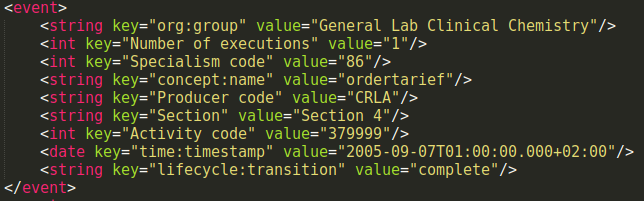
\includegraphics[width=\textwidth]{3_event_example.png}
		\caption{Trace example, exempt from the BPI11 hospital log~\cite{bpichallenge2011}}
		\label{figure:trace-example-1}	
	\end{center}
\end{figure}

One can see that the timestamp is present and one can define case id to be "Activity code" and activity ID as "concept:name".

There are number of other parameters such as "org:group" that shows the department in the clinic, "Number of executions" that shows number of times certain operation was performed and others.  All parameters combined give the best picture of the process execution, therefore it is important for methods exploiting logs to use most complete data set possible.

Furthermore, the logs can contain text information such as comments or emails, bringing up the complexity level of the problem. Text mining methods in conjunction with sequence classification should be used to bring down the problem~\cite{DBLP:conf/bpm/TeinemaaDMF16}.

As for example in the hospital log mentioned above, it might be a parameter with comments from the doctor for patient wellbeing. 

In the data based systems, the log can be stored in different structures. Enterprise Resource Planning (such as SAP, Oracle) systems have their own data format of journaling the data. It can also be CSV spreadsheet (figure~\ref{figure:trace-example-2_csv}) or XES formatted log (shown in figure ~\ref{figure:trace-example-1}).  

\begin{figure}[!ht]
	\begin{center}  
		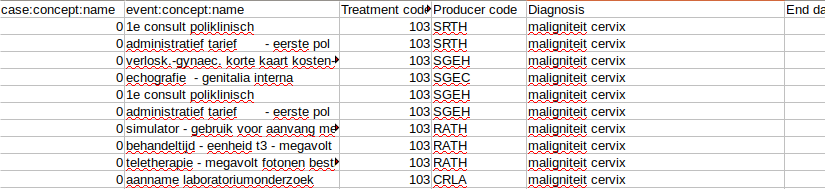
\includegraphics[width=\textwidth]{4_event_example_csv.png}
		\caption{Trace example (CSV format), exempt from the BPI11 hospital log~\cite{bpichallenge2011}}
		\label{figure:trace-example-2_csv}	
	\end{center}
\end{figure}



\subsection{Process mining}

\todo{More of this! }

Process mining is a business process management technique that enables the analysis of processes based on the event logs. The main idea is improving business processes based on analysis of the logs as sequential and continuous processes. This is what makes it different from the methods established in data mining and business intelligence which treat the data as set of distinct events to gather insights. 

As a rule the methods of process mining applied mostly to the processes that do not have formal description or have consistent deviations from the ones predicted in the system. 

The three main activities performed under the process mining field are:

\begin{itemize}
	\item \textbf{Process analysis (Discovery):} encompasses all methods to discover insights from the past process executions. As an example would be the issue to resolution process from the insurance company. Process discovery methods allow building abstract representation of an event log. The goal of this is to build approximated model that delivers better insights into the underlined processes. Discovered models can be in forms of BPMN models, Petri nets, and declarative rules. 
	\item \textbf{Conformance analysis:} it takes existent formalized models and check them against real log. In detail, that means that the business process analyst has the BPMN model for the process created (or generated). And now, the goal is to match the real processes to the model (mostly interest is in doing it on a fly). That is done in order to check for any deviations the process can have, and if possible to for prevention on undesired behavior.
	\item \textbf{Process enhancement:} it helps to use logs in order to enhance current executions of the processes. The information of the past is used to change the model and how the processes are being performed.
\end{itemize}
 


\subsection{Predictive monitoring}

Predictive monitoring is an advancing subfield of Process Mining. As a subfield of Process Mining, its main focus also lies in exploring and exploiting the process logs (the process executions). More specifically, predictive monitoring encompasses the methods that deal with online predictions of process outcomes. The outcome of interest can be compliance of with a measure (for example in an order to cash process the measure can be that any of the financial operations that involve an amount more then 2500 euro, are not performed without confirmation from the top financial officer), achieving objective (such as in issue to resolution process, if the process will be completed under 7 days time), or classifications (giving a label to the uncompleted trace, such as issue resolved, or not).  
\par
Many algorithms are applied to solve above mentioned problems, for example classic machine learning algorithms as classification and clustering~\cite{Leontjeva2015}. More complex concepts are also used, such as Markov models~\cite{Leontjeva2015}, time series~\cite{Lam20096986}, and deep learning~\cite{niek96732,evermann,quteprints96732} approaches. 
\par
In order to successfully apply these algorithms for facing the problems, it is necessary to have solid understanding on the process log nature. The aspects that can come into play, are the data types (while the case ID and activity ID are defined as categorical values, we have to deal with time stamps that are basically real valued, also text comments that are strings, or other numerical values such as sums of money), stationarity (it usually refers to time series data that have a stable mean, variance etc. over time. Best example from process logs are timestamps. One should account that they represent only the moment in an absolute time scale, while algorithms would only work if the input will be a relative measure, such as difference between timestamps). 
\par
Keeping in mind definition of the business process log from the section~\ref{logs} one can easily find the caveats in the early process mining approaches, that tend to ignore the data payload, taking into consideration only the control-flow (sequence of activities). Some of the approaches do the opposite, that is consider data, without control-flow~\cite{vanderAalst2010,DBLP:journals/is/AalstSS11,Schonenberg2008}. In that case the traces are considered to be a simple sequences. Moreover, methods introduced usually designed to work in offline fashion, exploring uncompleted cases. But, to make more accurate, mature, online predictions one should leave out neither payload nor control-flow information. That's when the Complex Symbolic Sequences as methods of encoding of a log are introduced. 


\subsection{Encodings of business logs}

Every machine learning problem needs the data represented in a particular way. To solve problem one needs to be aware that it is always a trade-off between the model used and the way of data encoding. 

In the next subsections the descriptions of the most used encodings are given.


\subsubsection{Simple symbolic sequence encoding}

This encoding is inherited from a massive number of works in machine learning and statistics such as concerning applications in health-informatics~\cite{Xing:2010:BSS:1882471.1882478}, or anomaly detection in Unix access systems, determining fraud users by its query log sequences. 

The simple symbolic sequence could be formalized as follows: $seq_{k} = (a_j)_{j=1}^{n}$.
Where the $seq_{k}$ is one trace in the log.


\begin{figure}[!ht]
	\begin{center}  
		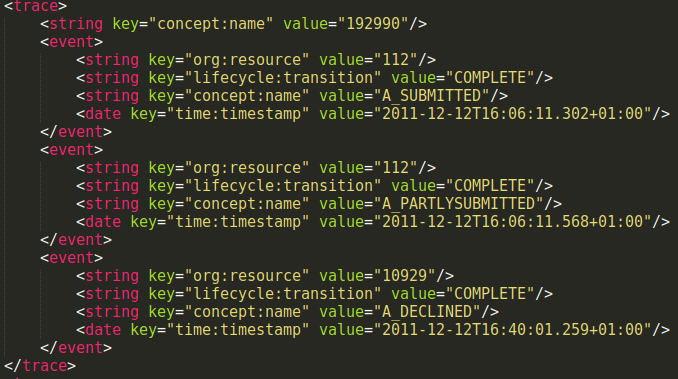
\includegraphics[width=\textwidth]{5_log_example_fin.png}
		\caption{Trace example, exempt from the BPI12 financial log~\cite{bpichallenge2012}}
		\label{figure:trace-example-2}	
	\end{center}
\end{figure}


As an example let's take a financial log from the bpi challenge. On the figure~\ref{figure:trace-example-2} one trace is shown.

So if we formalize this trace to the simple symbolic sequence from this log (considering activity ID to be "concept:name") it will have a form:

$seq = ("A\_SUBMITTED","A\_PARTLYSUBMITTED","A\_DECLINED")$

Simple Symbolic Sequences, however, have limitations that prevent getting best results of their use.

That is because simple symbolic sequences discard most of the rich information present in process logs, that is not limited to control-flow. An example would be the log in the big fast food chain, where the process about their employee's actions is daily recorded into the log. In Table~\ref{tab:statements}, you can see that log of this nature contains static features, control-flow components and number of dynamic features. Static feature include ID of the employee, and his age. Dynamic features are the $t_i$ that is the time spent working, $rID_i$ is an ID of the restaurant that employee worked in on that day, $rev_i$ money he earned for the company. 

\begin{table}[h]
	\centering
	\begin{tabular}{| l | l | l | l | l | l | l | l | l | l | l | l |}
		\hline
		& Age & ID & t\_1 & .. & t\_n & rID\_1 & .. & rID\_n & rev\_1 & .. & rev\_n \\	
		\hline
		tr1 & 20 & 00123 & 28800 & .. & 24840 & 11 & .. & 12 & 120\$ & .. & 112\$ \\
		tr2 & 24 & 00023 & 16890 & .. & 23460 & 12 & .. & 12 & 80\$ & .. & 111\$ \\
		tr3 & 18 & 01129 & 23804 & .. & 17897 & 11 & .. & 11 & 340\$ & .. & 23\$ \\
		tr4 & 21 & 00772 & 40034 & .. & 24564 & 12 & .. & 12 & 130\$ & .. & 2\$ \\
		\hline
	\end{tabular}
	\caption{Example of Complex Symbolic Sequence encoding}
	\label{tab:statements}
\end{table}


As well as the data used in areas described in the beginning on this chapter can be easily represented as simple symbolic sequence, there are many algorithms developed to work with. There are feature based classifications, sequence distance based, support vector machines, or model based classification~\cite{Xing:2010:BSS:1882471.1882478}. That's why first attempts to make predictions of the business processes were made with the use of this simple encodings.


\subsubsection{Complex symbolic encoding}

On contrary to Simple Symbolic Sequence encodings, the Complex Symbolic Sequences are introduced~\cite{Leontjeva2015} and we can capture much more information about log. Complex Symbolic Sequence is basically ordered list of vectors, where each vector is a subset of some alphabet inferred from the log.

When Complex Symbolic Sequences are used instead of Simple Symbolic Sequences for dealing with prediction problems, the complexity space of the prediction problem grows substantially. So it suggests to use new and more complex approaches to work with them.

Some of the base lines of working with complex symbolic sequences use index-based encodings, and index latest payload encodings mentioned in following paper~\cite{Leontjeva2015}.   

To exemplify this approach for encodings lets again take a look at the log in figure~\ref{figure:trace-example-2}. The Complex Symbolic Sequence form of this log will have following representation:

\begin{table}[h]
	\centering
	\begin{tabular}{| l | l | l | l | l | l | l | l | l |}
		\hline
		& $concept:n_{1}$ & .. & $concept:name_{3}$ & $org:resource_{1}$ & .. & $org:resource_{3}$ & $time:timestamp_{1}$ & .. \\	
		\hline
		tr1 & A\_SUBMITTED & .. & A\_DECLINED &  112 & .. & 10929 &  2011-12-12T16:06:11 & ..  \\
		tr2 &  & .. & .. & .. & .. & ..  & .. & ..  \\
		\hline
	\end{tabular}
	\caption{Example of Complex Symbolic Sequence encoding}
	\label{tab:complesymbseq_log_example}
\end{table}

This representation also has its downsides, even though it captures much more information. It is impossible to represent the complete log in this way, because one needs to limit the number of events in the traces to some definite number. In our example in the table~\ref{tab:complesymbseq_log_example} the trace length was chosen to be 3. 

This puts a limitation on the power of this encoding. The most use for the Complex Symbolic Encoding was found in~\cite{Leontjeva2015,Di-Francescomarino:2016aa,DBLP:conf/bpm/TeinemaaDMF16}. They used it for binary classification of traces. 



\subsubsection{One-hot encoding} \label{one-hot-encoding}

As more advanced machine learning methods were brought to process mining, such as family of deep learning neural networks~\cite{evermann,niek96732,quteprints96732,evermann2}. With them came the new ways of representing the process log.

This is actually the v×m sized matrix, where each row represents one step of business process. One-hot is because the table can only contain the binary value of one or zero. (even though some extended versions of one-hot encoding are used to add information of features such as time~\cite{niek96732}). 

Even though the table is usually large and not so efficient memory-wise, but is best for neural networks computations (as most of the operations are multiplications, it's easy to multiply and add ones and zeros). 

In we turn the log from the figure~\ref{figure:trace-example-2} into the one-hot encoding it will have representation shown in table~\ref{tab:one-hot} (we use only control-flow in this example, that is the activity ID).

\begin{table}[h]
	\centering
	\begin{tabular}{| l | l | l | l |}
		\hline
		& A\_SUBMITTED & A\_PARTLYSUBMITTED & A\_DECLINED \\	
		\hline
		$e_{1}$ & 1 & 0 & 0 \\
		$e_{2}$ & 0 & 1 & 0 \\
		$e_{3}$ & 0 & 0 & 1 \\
		\hline
	\end{tabular}
	\caption{Example of One-hot encoding}
	\label{tab:one-hot}
\end{table}



\subsection{RNNs and LSTM}
Artificial Neural Networks (or just Neural Networks, NNs) are a well
known class of discriminative models. In classification tasks, they are
used to model the probability of a given input to belong to a certain
class, given some features of the input. We can describe them in
mathematical terms as follows:
%
\begin{equation}
  \label{eq:condprob}
  p(\mathbf{y}|\mathbf{x}) = f_{\mathit{NN}}(\mathbf{x}; \theta).
\end{equation}
%
In \eqref{eq:condprob}, $\mathbf{x}$ is the feature vector that represents the input,
$\mathbf{y}$ is a random variable representing the output class
labels, $f_{\mathit{NN}}$ is the function modeled by the neural network, and
$\theta$ is the set of parameters of such a function to be learnt during
the training phase.


\begin{figure}[t]
  \centering
  \resizebox{.56\textwidth}{!}{
    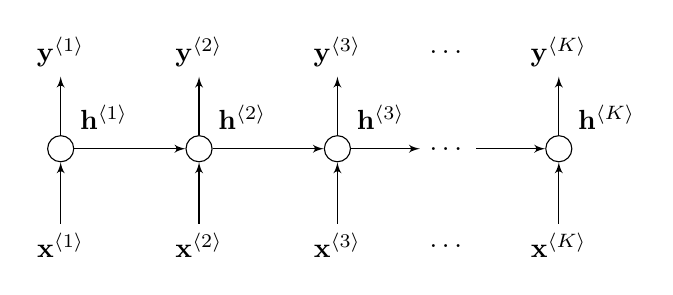
\begin{tikzpicture}[node distance=5em]
	% \matrix [column sep={6em,between origins},row sep=4em]
	% {
      \node [name=x_1] {$\mathbf{x}^{\langle 1 \rangle}$};
      \node [name=x_2, right of=x_1] {$\mathbf{x}^{\langle 2 \rangle}$};
      \node [name=x_3, right of=x_2] {$\mathbf{x}^{\langle 3 \rangle}$};
      \node [name=x_dots, right of=x_3, xshift=-1em] {\ldots};
      \node [name=x_K, right of=x_dots, xshift=-1em] {$\mathbf{x}^{\langle K \rangle}$};

      \node [draw, shape=circle, name=h_1, above of=x_1, yshift=-1.5em, label=above right:{$\mathbf{h}^{\langle 1 \rangle}$}] {};
      \node [draw, shape=circle, name=h_2, above of=x_2, yshift=-1.5em,label=above right:{$\mathbf{h}^{\langle 2 \rangle}$}] {};
      \node [draw, shape=circle, name=h_3, above of=x_3, yshift=-1.5em,label=above right:{$\mathbf{h}^{\langle 3 \rangle}$}] {};
      \node [name=h_dots, above of=x_dots, yshift=-1.5em] {\ldots};
      \node [draw, shape=circle, name=h_K, above of=x_K, yshift=-1.5em, label=above right:{$\mathbf{h}^{\langle K \rangle}$}] {};

      \path [draw, -latex'] (x_1.north) -- (h_1.south);
      \path [draw, -latex'] (x_2.north) -- (h_2.south);
      \path [draw, -latex'] (x_3.north) -- (h_3.south);
      \path [draw, -latex'] (x_K.north) -- (h_K.south);

      \node [name=y_1, above of=h_1, yshift=-1.5em] {$\mathbf{y}^{\langle 1 \rangle}$};
      \node [name=y_2, above of=h_2, yshift=-1.5em] {$\mathbf{y}^{\langle 2 \rangle}$};
      \node [name=y_3, above of=h_3, yshift=-1.5em] {$\mathbf{y}^{\langle 3 \rangle}$};
      \node [name=y_dots, above of=h_dots, yshift=-1.5em] {\ldots};
      \node [name=y_K, above of=h_K, yshift=-1.5em] {$\mathbf{y}^{\langle K \rangle}$};

      \path [draw, -latex'] (h_1.north) -- (y_1.south);
      \path [draw, -latex'] (h_2.north) -- (y_2.south);
      \path [draw, -latex'] (h_3.north) -- (y_3.south);
      \path [draw, -latex'] (h_K.north) -- (y_K.south);

      \path [draw, -latex'] (h_1.east) -- (h_2.west);
      \path [draw, -latex'] (h_2.east) -- (h_3.west);
      \path [draw, -latex'] (h_3.east) -- (h_dots.west);
      \path [draw, -latex'] (h_dots.east) -- (h_K.west);
      % }
    \end{tikzpicture}
  }
  \caption{Recurrent Neural Network}
  \label{fig:rnn}
\end{figure}

Recurrent Neural Networks (RNNs, see Fig.~\ref{fig:rnn}) are a subclass of Neural Networks. We
illustrate them with the help of an example in which the
classification task concerns the assignment of correct part of speech -- noun, verb, adjective, etc. --
to words.  If we take the word \emph{``file''} in isolation,
it can be both a noun and a verb. Nonetheless, this ambiguity
disappears when we consider it in an actual sentence. Therefore, in the
sentence \emph{``I have to file a complain''} it acts as a verb, while
in the sentence \emph{``I need you to share that file with me''} it
acts as a noun.

This simple example shows that for some tasks the classification at a
certain time-step $t$ depends not only on the current input (i.e.,
\emph{``file''}) but also on the input (i.e., the part of the
sequence) seen so far. The tasks that share this characteristic are
said to be \emph{recurrent}. Natural Language tasks are a typical
example of recurrent phenomena.

In mathematical terms, let us write
$\mathbf{x}^{\langle 1 \rangle}, ..., \mathbf{x}^{\langle K \rangle}$
to indicate an input sequence of $K$ time-steps, represented by the
superscript between angle brackets. In this way, at each time-step $t$,
the conditional probability of a given input to belong to a certain class is described by
%
\begin{equation}
\label{eq:condprobrec}
  p(\mathbf{y}^{\langle y \rangle}|\mathbf{x}^{\langle t \rangle}, ..., \mathbf{x}^{\langle 1 \rangle}) = f_{\mathit{RNN}}(\mathbf{x}^{\langle 1 \rangle}, ..., \mathbf{x}^{\langle t \rangle}; \theta).
\end{equation}
%
\todo{Add example}
RNNs have been proven to be extremely appropriate for modeling sequential
data (see~\cite{goodfellow2016dlbook}). As shown in Fig.~\ref{fig:rnn}, they typically leverage
recurrent functions in their hidden layers, which are, in turn, composed of hidden states. Let
$\mathbf{h}^{\langle t \rangle}$, with
\begin{equation}
  \label{eq:hidden}
  \mathbf{h}^{\langle t \rangle} = h(\mathbf{x}^{\langle t \rangle}, \mathbf{h}^{\langle t-1 \rangle}; \theta_{h});
\end{equation}
be the activation of the hidden state at the $t$-th time-step. $h$ is a so-called \emph{cell function}, parameterized over a set
of parameters $\theta_{h}$ to be learnt during the training, and accepting as inputs the current input $\mathbf{x}^{\langle t \rangle}$ and its value at the
previous time-step $\mathbf{h}^{\langle t-1 \rangle}$.
The activation of the hidden state is then mapped (using a linear map) into a continuous vector of the
same size as the number of output classes. All the elements in such a vector are greater than zero and their sum is equal to one. Therefore, this vector can be seen as a probability distribution over the output space.
All these constraints can be easily achieved specifying the generic equation \eqref{eq:condprobrec} by means of a softmax function:
%
\begin{equation}
  \label{eq:softmax}
  p(\mathbf{y}^{\langle y \rangle}|\mathbf{x}^{\langle t \rangle}, ..., \mathbf{x}^{\langle 1 \rangle}) =
  softmax(\mathbf{W}\mathbf{h}^{\langle t \rangle} + \mathbf{b});
\end{equation}
%
where the weight matrix $\mathbf{W}$ and the bias vector $\mathbf{b}$
are parameters to be learnt during the training phase.

% The presentation of RNNs ends with a note about the representation of the input: at each time-step, the
% input should be represented by means of a vector. When our input space is
% made of a finite set of symbols (e.g. a vocabulary of words) the most
% straightforward way to represent it is to use a one-hot encoding:
% the $i$-th symbol will be encoded into a vectors of dimension equal to
% the dimension of the input space with all the elements set to 0 and
% just the $i$-th to one. Such representations are not very practical:
% they grow linearly with the dimension of the input space; their sum produce a vector which is not one-hot anymore; multiplying them
% element-wise produce an all-zero vector; and so on. To overcome such limitations, the so called \emph{low
%   dimensional embedding} technique is used: the $i$-th symbol is
% represented with the $i$-th row of an \emph{embedding matrix} learnt
% at training time. The number of the column of the matrix, and
% consequently the dimension of the input vectors, is an hyper-parameter
% of the model to be set at design time.

Among the different cell functions $h$ (see equation~\eqref{eq:hidden}) explored in the literature, Long Short-Term
Memory (LSTM)~\cite{hochreiter1997long} shows a significant ability to maintain the memory of its input across long time spans. This property makes them extremely suitable to be used in RNNs that have to deal with input sequences with complex long-term dependencies such as the ones we consider in this thesis.

% The cell made of four \emph{gates}, namely the input gate $\mathbf{i}$, the forget gate $\mathbf{f}$, the output gate $\mathbf{o}$ and the cell update gate $\mathbf{g}$.
% At each time step, we have that:
% \begin{equation}
%   \label{eq:lstmgates}
%   \begin{aligned}
%     \mathbf{i}^{\langle t \rangle} &= \sigma(\mathbf{W}_i\mathbf{x}^{\langle t \rangle} + \mathbf{U}_i\mathbf{h}^{\langle t-1 \rangle} + \mathbf{b}_i);\\
%     \mathbf{f}^{\langle t \rangle} &= \sigma(\mathbf{W}_f\mathbf{x}^{\langle t \rangle} + \mathbf{U}_f\mathbf{h}^{\langle t-1 \rangle} + \mathbf{b}_f);\\
%     \mathbf{o}^{\langle t \rangle} &= \sigma(\mathbf{W}_o\mathbf{x}^{\langle t \rangle} + \mathbf{U}_o\mathbf{h}^{\langle t-1 \rangle} + \mathbf{b}_o);\\
%     \mathbf{g}^{\langle t \rangle} &= f(\mathbf{W}_g\mathbf{x}^{\langle t \rangle} + \mathbf{U}_g\mathbf{h}^{\langle t-1 \rangle} + \mathbf{b}_g);\\
%   \end{aligned}
% \end{equation}
% where
% $\theta_{LSTM} = [\mathbf{W}_i, \mathbf{U}_i, \mathbf{b}_i,
% \mathbf{W}_f, \mathbf{U}_f, \mathbf{b}_f, \mathbf{W}_o, \mathbf{U}_o,
% \mathbf{b}_o, \mathbf{W}_g, \mathbf{U}_g, \mathbf{b}_g]$ is the set of
% parameters to be learned during the training phase.  The cell holds an
% internal state $\mathbf{c}^{\langle t \rangle}$ that is updated at
% each timespep according to the following:
% \begin{equation}
%   \label{eq:lstmstate}
%   \mathbf{c}^{\langle t \rangle} = \mathbf{f}^{\langle t \rangle} \odot \mathbf{c}^{\langle t-1 \rangle} + \mathbf{i}^{\langle t \rangle} \odot \mathbf{g}^{\langle t-1 \rangle};
% \end{equation}
% being $\odot$ the element-wise product between two vectors,
% $\sigma(\cdot)$ the sigmoid function and $f(\cdot)$ a non-linear
% function, typically the hyperbolic tangent $\tanh(\cdot)$. Intuitively
% we can see how the forget gate $\mathbf{f}$ controls how much of the
% previous cell state flows into the current state, while the input gate
% controls how much of the cell update signal gets into it. Finally, the
% cell activation is given by the:
% \begin{equation}
%   \label{eq:lstmactivation}
%   \mathbf{h}^{\langle t \rangle} = \mathbf{o}^{\langle t \rangle} \odot f(\mathbf{c}^{\langle t \rangle});
% \end{equation}
% where the output gate controls the fraction of output signal coming from the cell state.

\subsection{RNNs with LSTM for Predictive Process Monitoring}
\label{subsec:RNNforpredictive}
In order to provide predictions on the suffix of a given prefix (of a running case), state-of-the-art approaches for predictive process monitoring use RNNs with LSTM cells.  The most recent and performing approach in this field \cite{niek96732} relies on an encoding of activity sequences that combine features related to the activities in the sequence (the so called \textit{one-hot encoding}, described in section ~\ref{one-hot-encoding}) and features related to the time characterizing these activities. Given the set $A = \{a_{1_A}, \ldots a_{m_A}\}$ of all possible activities, an ordering function $idx:A \rightarrow \{1, \ldots, \left|A\right| \} \subseteq \mathbb{N}$ is defined on it, such that $a_{i_A}<>a_{j_A}$ if and only if $i_A<>j_A$, i.e., two activities have the same A-index if and only if they are the same activity. For instance, if $A=\{a,b,c\}$, we have $idx: A \rightarrow \{1,2,3\}$ and $idx(a)=1$, $idx(b)=2$ and $idx(c)=3$. Each activity $a_i \in \sigma$ is encoded as a vector $\mathbb(A_i)$ of length $|A|+3$ such that the first $|A|$ features are all set to $0$, except the one occurring at the index of the current activity $idx(a_i)$, which is set to $1$. The last three features of the vector pertain to time: the first one relates to the time increase with respect to the previous activity, the second reports the time since midnight (to distinguish between working and night time), and the last one refers to the time since the beginning of the week.
%For example, given the alphabet $A$ above, the activity $b$ in a trace $\sigma =  \left\langle bcc \right\rangle$ will be encoded as the vector $(0,1,0)$.

A trace is encoded by composing the vectors obtained from all activities in the trace into a matrix. During the training phase, the encoded traces are used for building the LSTM model. During the testing phase, a (one-hot encoded) prefix of a running case is used to query the learned model, which returns the predicted suffix by running an inference algorithm.
%\todocdf{Do we need other details about the architecture?}
Algorithm~\ref{alg:baseline} reports the inference algorithm introduced in \cite{niek96732} and based on RNN with LSTM cells for predicting the suffix of a given prefix $p_k(\sigma)$ of length $k$. The algorithm takes as input the prefix $p_k(\sigma)$, the LSTM model $lstm$ and a maximum number of iterations $max$ and returns as output the complete trace (the prefix and the predicted suffix).
First, the prefix $p_k(\sigma)$ is encoded by using the one-hot encoding (line~\ref{lst1:encoding}). The resulting matrix is then used for feeding the LSTM model and getting the probability distribution over different possible symbols that can occur in the next position of the trace (line~\ref{lst1:prob}). The symbol with the highest probability is hence selected from the ranked probabilities (line~\ref{lst1:next}). Then, a new trace is obtained by concatenating the current prefix with the new predicted symbol (line~\ref{lst1:trace}). In order to predict the second activity, the one-hot encoding of the new prefix is computed and used to recursively feed the network. The procedure is iterated until the predicted symbol is the end symbol or a maximum number of iterations $max$ is reached (line~\ref{lst1:while}).

\begin{algorithm}
	\caption{Inference algorithm for predicting the suffix of $p_k(\sigma)$}
	\label{alg:baseline}
	\begin{algorithmic}[1]
		\Function{PredictSuffix}{$p_k(\sigma)$, $lstm$, $max$}
		\State $k$ = 0
		\State $trace$ = $p_k(\sigma)$
		\Do
		\State $trace_{encoded}$ = \textsc{encode}($trace$) \label{lst1:encoding}
		\State $next\_symbol\_probs$ = \textsc{predictNextSymbols}($lstm$, $trace_{encoded}$) \label{lst1:prob}
		\State $next\_symbol$ = \textsc{getSymbol}($next\_symbol\_prob$, $trace_{encoded}$) \label{lst1:next}
		\State $trace$ = $trace \cdot next\_symbol$\label{lst1:trace}
		\State $k = k + 1$
		\doWhile{$($not $next\_symbol$ == $end\_symbol)$ and $(k$ \textless $max)$}\label{lst1:while}
		\State \textbf{return} $trace$
		\EndFunction
	\end{algorithmic}
\end{algorithm}

%\begin{algorithm}[H]
%	\KwData{$p_k(\sigma)$}
%	\KwResult{$\sigma$}
%	initialization\;
%	\While{end symbol not predicted}{
%		enc = encode-one-hot ($p_k$)\;
%		prob-distr = model.predict(enc)\;
%		predicted = choose most probable(prob-distr)\;
%		$p^{k+1}$ = concatenate $p_k(\sigma)$ + predicted\;
%		k = k + 1\;
%	}
%	return $p_k$
%	\caption{Inference in RNN for predicting the suffix of a prefix of $k$ symbols}
%	\label{alg:baseline}
%\end{algorithm}

%\todocdf{Which one shall we keep?}

%\begin{algorithm}
%	\caption{Baseline inference algorithm for predicting suffix of activities}
%	\label{alg:baseline}
%	\begin{algorithmic}[1]
%		\Function{EvaluateSuffix}{$prefix$, $model$, $limit$}
%		\State $k$ = 0
%		\State $traceResulting$ = $prefix$
%		\Do
%		\State $encoded$ = encode($traceResulting$)
%		\State $nextSymbolProb$ = predictNext($model$,$encoded$)
%		\State $nextSymbol$ = getSymbol($nextSymbolProb$)
%		\State $traceResulting$ = concatenate($traceResulting$, $nextSymbol$)
%		\State k = k + 1
%		\doWhile{$($not $nextSymbol$ equal to $endSymbol)$ and $(k$ \textless $limit)$}
%		\State return traceResulting
%		\EndFunction
		
%		\Function{getSymbol}{$nextSymbolProb$}
%		\State top = chooseMaxProb($nextSymbolProb$)
%		\State return probabilityToSymbol(top)
%		\EndFunction
		
%	\end{algorithmic}
%\end{algorithm}




\subsection{Linear Temporal Logic}

Linear Temporal Logic~\cite{Pnueli77} (LTL) is a modal logic with modalities devoted to describe time aspects. Classically, LTL is defined for infinite traces. However, to describe the characteristics of a business process, we use a variant of LTL defined for finite traces (since business processes are supposed to complete eventually).
%
We assume that activities occurring during the process execution fall into the set of atomic propositions. LTL rules are constructed from these atoms by applying the temporal operators $\NEXT$ (next), $\sometime$ (future), $\always$ (globally), and $\until$ (until) in addition to the usual boolean connectives. Given a formula $\varphi$, $\NEXT \varphi$ means that the next time instant exists and $\varphi$ is true in the next time instant (strong next). $\sometime \varphi$ indicates that $\varphi$ is true sometimes in the future. $\always \varphi$ means that $\varphi$ is true always in the future. $\varphi \until \psi$ indicates that $\varphi$ has to hold at least until $\psi$  holds and $\psi$ must hold in the current or in a future time instant.

\subsection{Beam search}

Beam search is a heuristic search algorithm, based on the principle of exploring the graph of possible solutions by the most promising node. It is built for dealing with huge search spaces. Specifically, it orders all partial solutions with some heuristic measure; it then keeps only a small portion of the most promising solution, and expands them to get the complete solution.

Beam search is used in area such as machine translation\cite{Koehn2007MOSEStranslationSystem}.


There are few variants of this algorithm, two of which will be thoroughly explained here: The best-first and the breadth-first. 

\subsubsection{Best-first variation of Beam search}

Best-first search explores the solution space following the most probable solution first. The algorithm exploits a tree structure, in which each node maintains its state as open and closed (open state means that the node of the tree was not visited yet, and can be explored in the next iteration, while closed means that the node was already visited). The algorithm assumes that all nodes are open at the initialization and, after visiting the nodes marks them as closed. 

The pseudo code for the algorithm described in the listing~\ref{alg:bestfirst}.


\begin{algorithm}
	\caption{Best first search}
	\label{alg:bestfirst}
	\begin{algorithmic}[1]
		\State define node of the graph, OPEN, to be starting node $s$
		\If {\textsc{list} is empty} 
		\State	failure
		\EndIf
		\State Take the best node from the list (call it $n$), and make it CLOSED
		\State Expand node $n$
		\If {any of the successor nodes are the solution} 
			\State	success, return the solution traced back
		\EndIf
		\ForAll {node of the successors} 
		\State	apply evaluation function $f$ to the $node$\;
		\State	if $node$ is new (not CLOSED) mark as OPEN\;
		\EndFor
	\end{algorithmic}
\end{algorithm}


On the first line, the graph is initialized, and next the list is checked if it's empty. On the fifth line the nodes from the list are ordered, and top one is chosen. The line 6, algorithm takes the top node for further processing. The 7-9 lines state if the solution found, the algorithm should construct the solution by tracing back the tree by parent nodes and return it. Lines 10-13 state that if the solution is not found, we take all nodes from successors of n, and apply the evaluation function, and if this new node is new to the algorithm (not yet exploited) we mark it as open.

Different evaluation functions can be used for the task. The decision is made upon the specifics of the problem, and it directly influences the effectiveness of an algorithm. The example of the evaluation function can be the count of events if we need the prediction to be short, or if the predicted sequence is conformant with defined rule.

\subsubsection{Breadth-first variation of Beam search}

Breadth-first search begins with an empty node and explores the search space in the breadth-wise order. This type of beam search operates using few priority queues instead of tree structures as in the previous approach. 

Algorithms reported in the pseudo code listing~\ref{alg:breathfirst} (all elements in priority queues are stored with priority based on some evaluation function)

The algorithm starts with defining two priority queues on the line 1. On the line 2, first queue is appended with the element given as an input. Third line defines the condition that calculations will stop that is if the solution tree has reached its bottom. Line 4 starts the while loop that will iterate over all elements in s1. Lines 5-9 describe that each element from $s1$ either a solution (in that case line 7 returns it), or the next elements are predicted and top $beamsize$ elements are chosen to be passed to the next iteration.


\begin{algorithm}
 	\caption{Breath-first Beam search}
	\label{alg:breathfirst}
	\begin{algorithmic}[1]
		\State define two empty priority queues, $s1$ and $s2$
		\State add the first element to $s1$
		\While {solution is not found or the search space is not empty} 
			\While {s1 is not empty}
				\State get element $elem$ from s1
				\If{ solution found } 
					\State	success
					\EndIf
					\State expands $elem$ and write $beamsize$-elements to s2
					\EndWhile
					\State $s2$ equals first part of $s1$ with the size of $beamsize$
					\EndWhile
	\end{algorithmic}
\end{algorithm}




\vspace{0.2 cm}
Both the beam search algorithms use the same tactic: they cut the search space as to keep only the most probable and better performing prospective solutions. These algorithms are different, and depending on the nature of the problem given can have very different performance.



% section background (end)

%%% Local Variables:
%%% mode: latex
%%% TeX-master: "BPM17"
%%% End: 




\section{Related Work} % (fold)
%!TEX root = ./BPM17.tex
\label{sec:related_work}

The literature related to predictive business process monitoring can be roughly classified according to the type of predictions that is provided.
A first group of works focuses on the time perspective. In~\cite{DBLP:journals/is/AalstSS11}, the authors present a set of approaches in which annotated transition systems, containing time information extracted from event logs, are used to: (i) check time conformance;
  (ii) predict the remaining processing time of incomplete cases; (iii) recommend appropriate activities to end users working on these cases. In \cite{Folino}, an approach for predicting business process performances is presented. The approach is based on context-related execution scenarios discovered and modeled through state-aware performance predictors. In~\cite{DBLP:conf/icsoc/Rogge-SoltiW13}, the authors use stochastic Petri nets to predict the remaining execution time of a process execution. In~\cite{Metzgeretal12}, the authors present a technique for predicting the delay between the expected and the actual arrival time of cases pertaining to a transport and logistics process. In~\cite{Senderovichetal15}, the queue theory is used in order to predict possible delays in process executions.

Another set of works in the literature focuses on approaches that generate predictions and recommendations to reduce risks. For example, in~\cite{DBLP:conf/caise/ConfortiLRA13}, the authors present a technique to support process participants in making risk-informed decisions with the aim of reducing the process risks. Risks are predicted by traversing decision trees generated from the logs of past process executions. In~\cite{Pika}, the authors make predictions about time-related process risks by identifying and leveraging statistical indicators observable in event logs  that highlight the possibility of transgressing deadlines.
In \cite{suriadi}, an approach for Root Cause Analysis through classification algorithms is presented.

A third group of prediction approaches predicts the outcome (e.g., the satisfaction of a business objective) of a case. In~\cite{Maggi:CAiSE2014} a framework is introduced, which is able to predict the fulfillment (or the violation) of a boolean predicate in a running case, by looking at: (i) the sequence of activities already performed in the case; and (ii) the data payload of the last activity of the running case. The framework, which provides accurate results at the expense of a high runtime overhead, has been enhanced in~\cite{Di-Francescomarino:2016aa} by introducing a clustering preprocessing step in which cases sharing a similar activity history are clustered together. A classifier for each cluster is trained with the data payload of the traces in the cluster. In~\cite{Leontjeva2015}, the authors compare different feature encoding approaches where traces are treated as complex symbolic sequences, that is, sequences of activities each carrying a data payload consisting of attribute-value pairs. In~\cite{DBLP:conf/bpm/TeinemaaDMF16}, the unstructured information contained in text messages exchanged during process executions has been leveraged for improving the prediction accuracy.

The problem investigated in this paper falls into a fourth and last set of works, i.e., into the set of very recent efforts aiming at predicting the sequence of future activities given the activities observed so far.
%~\cite{Polatoetal:2016,niek96732,evermann}.
In~\cite{Polatoetal:2016}, Polato et al.~propose several techniques for predicting the remaining time and the sequence of future activities in an ongoing case using simple regression, regression with contextual information, and data-aware transition systems.
%
%Recently, many machine learning toolkits started leveraging the power
%of Graphical Processing Units (GPUs).  This allowed researchers and
%engineer to train their NNs in a significantly reduced amount of time:
%many complex network architectures have been trained to perform
%several task, many of them achieving remarkable performances.  Such
%innovation fostered a new interest in NNs that spread across both
%Industry and Industry.  Business Process Management is not an
%exception. \cite{quteprints96732,niek96732,evermann} Recent papers
%suggest state of the art performance on the prediction tasks for
%business process log outcomes.
%
%Due to the nature of the problem, that is the sequence to sequence prediction, the recurrent neural networks are most leveraged. The main motivation for this type of neural networks is currently the problems in Natural Language Processing, such as speech recognition\cite{graves2013icassp}, or translation\cite{Sutskever2014SSL29690332969173}.
%
% In ~\cite{quteprints96732}, Verenich et al. rely on RNNs with sliding windows for predicting the next activity, i.e., they use $k$events to predict the event $k+1$.% (to predict event k+1, they use k..(N+k) events).
Other approaches~\cite{evermann,niek96732} make use of RNNs with LSTM cells.
In particular, Evermann et al.~\cite{evermann} propose an RNN with two hidden layers trained with back propagation,  %, 500 dimensions and 20 steps. They use batches of 20 to train the RNN with back propagation.
%The evaluation was made on the BPI2012, BPI2013 data sets. They argue that the results with this approach are comparable to state of the art based on clustering and annotating transition system approaches.
while Niek et al.~\cite{niek96732} leverage LSTM and an encoding based on activities and timestamps (illustrated in detail in Section~\ref{subsec:RNNforpredictive}) to provide predictions on the next activities and their timestamps.
% The results show that their approach, which is the most recent one in the literature, outperforms all the others.
Differently from all these works, this paper investigates how to take advantage of possibly existing a-priori knowledge for making predictions on the sequence of future activities.

%\todoincg{Fix bibentry for Niek. I would cite the technical report from which we took the data adding as a note that a version is to appear in CAISE 2017.}

%They achieve state of the art performance on most logs evaluated.
%In order to predict the next events and their timestamps, they rely on a boolean encoding of the event sequences and on few time-related features. The encoding is then used for feeding the RNN.

%In order to predict next event and time, they use one-hot encoding for event sequence, and few time features (such as difference between time-stamps, time from midnight, time from beginning of the week). Using these features they construct a vector to be fed into recurrent neural network.

%They are looking for functions $f_a^1$ and $f_t^1$ that are basically the probability distributions over all possible trace continuations.

%Also, as they now have basically two sequences to train with, that are the sequence of events, and the sequence of time values, the paper suggests the different possible RNN architectures.
%\begin{figure}[!ht]
%	\begin{center}
%		\includegraphics[width=\textwidth]{paper1233.png}
%		\caption{Possible neural network architectures \cite{niek96732}. Single task layers (a), shared multitask layers (b), or n+m shared layers (c).}
%	\end{center}
%\end{figure}

%The evaluation was done on many data sets, such as Helpdesk, BPI12, BPI12 with no duplicates, Environment permit. On most of them suffix (sequence of next events) prediction beats state of the art performance. It worked especially well with logs that had a lot of short traces (Helpdesk log contains average 7 event traces).
%%% Local Variables:
%%% mode: latex
%%% TeX-master: "BPM17"
%%% End:

%!TEX root = ./BPM17.tex

\section{The Problem} % (fold)
\label{sec:the_problem}
%%%% CONTENT
% general problem of predicting with background knowledge
Predictive business process monitoring methods use past process executions, stored in event logs, in order to build predictive models that work at runtime to make predictions about the future.
Among the different types of predictions about an ongoing case, such as the remaining time or the fulfilment of a predicate, we can find the prediction of the sequence of future activities. This type of predictions can be useful in the scenario where some planning and resource allocation are needed for the running case.
%For instance, a call center is strongly interested in predicting future activities of its customers to be able to adopt the best strategy for convincing them to buy a product.
For instance, the hospital management can be highly interested in predicting the future activities of patients to be able to best organize machines and resources of the hospital.



Nonetheless, predicting sequences of activities is a quite complex and challenging task, as the longer the sequence is, the more difficult is to predict the most far-away activities.
%In these scenarios the history of past customers can be leveraged to learn about the future of current customers.
%This is mainly due to the fact that the longer the sequence is, the more difficult is predicting the most far-away activities.
While predicting the sequence of future activities entirely from past execution data may be difficult, in real world scenarios, we often observe that some a-priori knowledge about the future of the running process executions exists and could hence be leveraged to support the predictive methods and improve their accuracy.

%For instance, the call center can already know that no customer will buy a given product as it is not anymore available, or that a specific customer will buy a specific product as it has already assessed it.

For instance, in the hospital example, new medical guidelines may provide new knowledge on the fact that two treatments are not useful if used together in order to cure a certain disease, or that a certain screening is required in order to perform a specific surgery, or also that if a patient is allergic to a specific treatment she will never go to take it.

Also the exemplary knowledge known a-prior might be the weather information for the agricultural company that does the harvest. Knowledge about problems with diesel supplies can help a company to project on how their real processes concerning harvesting will unfold. For example assuming they are having delays with a supply in the middle of harvesting season, the big machinery usually used will not be able to perform needed operations. So inferring the incapability to use them will help to predict the real unfold of the processes. That could help the management to guide their choices to best account for the new circumstances. 


Moreover if the algorithmically this problem could be accurately solved it can bring much more benefits to the companies. It can be also used for simulation purposes. For example a big insurance company, that deals with thousands claims per day could decide that they need some changes such as cutting down jobs. Now they will have a capability to predict what will happen under the assumption of job cuts, and that could provide better insights. So besides classical qualitative methods of business process management that use BPMN models to analyze the changes my means of queuing theory or simulation, one would have one more instrument in the toolkit. This algorithm would enable a process owner to use some proposed changes as a-priori knowledge, and after predicting the continuations of the traces make further analysis. 

Given the practical motivations for the problem at hand let's dive once more into the research question identified.

RQ: How can prior knowledge about an ongoing case be used to boost accuracy of predictions of trends of activities?

Here we decompose the research question into chunks to better understand the problem stated. \textit{Boost accuracy of prediction} means to develop an approach that will have better performance than current state of the art. \textit{Trends of activities} means that we are interested in finding the suffix of the current ongoing process execution. \textit{Ongoing process} means that we will have \textit{prior knowledge} on the inference time. 





This a-priori knowledge can be expressed in terms of LTL rules. For instance, in the hospital example, LTL can be used for defining the following rules:
\begin{enumerate}[1)]
\item \texttt{treatmentA} and \texttt{treatmentB} cannot be both used within the same course of cure of a patient:
  \begin{equation}
    \label{eq:LTL1}
    \neg(\sometime \mathtt{treatmentA} \wedge \sometime \mathtt{treatmentB})
  \end{equation}
\item \texttt{screeningC} is a pre-requisite to perform \texttt{surgeryD}:
  \begin{equation}
    \label{eq:LTL2}
    (\neg \mathtt{surgeryD} \until \mathtt{screeningC}) \vee \always (\neg  \mathtt{surgeryD})
  \end{equation}
\item \texttt{treatmentB} cannot be performed on this course of cure (e.g., because the patient is allergic to it):
\begin{equation}
	\label{eq:LTL3}
	\neg \sometime \mathtt{treatmentB}
\end{equation}
\end{enumerate}

In this paper, we aim at understanding whether and how a-priori knowledge can be leveraged in order to improve the accuracy of the prediction of the (sequence of the) next activity(ies) of an ongoing case in a reasonable amount of time. For instance, in the example of the hospital, being aware of the fact that \texttt{treatmentA} and \texttt{treatmentB} can never be executed together could help in ruling out a prediction of \texttt{treatmentB} whenever we have already observed \texttt{treatmentA} and vice versa.
%the problem of predicting the sequence of future activities consists of identifying the function $f(p_k(\sigma)) = s^k(\pi_A(\sgigma))$. When some a-priori knowledge $k(\sigma)$ for the (set of) ongoing trace is available, we are interested in identifying the function $f(p_k(\sigma), k(\sigma)) = s^k(\pi_A(\sigma))$

%For example, it is easy to express simple rules such as "eventually will happen 'A'", or "After 'A' follows 'B'".

%Beyond the information gathered from the sequence of events (and associated payloads), other types of information can be leveraged in order to boost the accuracy of the prediction. For instance, specificities can exist in the structure of the data, which , it can happen that,  some a-priori knowledge about the future of the running process execution exists and could hence be leveraged to support the predictive methods and improve their accuracy.

% how to predict, how to predict when you know that your dataset is "loopy", how do you predic with background knowledge?
%In this paper we would like to investigate the following questions:
%\begin{itemize}
%\item how do we predict the next activity(ies) by leveraging knowledge from the past?
%\item how do we enhance the prediction of the next activity(ies) by also leveraging knowledge on the structure of the data?
%\item how do we enhance the prediction of the next activity(ies) by also leveraging apriori knowledge on the future?
%\end{itemize}

%In the following section we focus on these three research questions
% section the_problem (end)

Formally, given a prefix $p_k(\sigma)=\left\langle a_1, ..., a_k\right\rangle$ of length $k$ of a trace $\sigma=\left\langle a_1, ..., a_n\right\rangle$ and some knowledge $\cal{K}(\sigma)$ on $\sigma$, the problem we want to face is to identify the function $f$ such that $f(p_k(\sigma), \cal{K}(\sigma))$ = $s_k(\sigma)$.

%!TEX root = ./BPM17.tex

\section{The Solution} % (fold)
\label{sec:our_approach}
%%%% CONTENT
% subsection 1: loops
% subsection 2: background K

% section our_approach (end)
%Our objective is to predict sequences of activities, by taking into account available a-priori knowledge, in a reasonable amount of time.
%the next activity and the sequence of next activities of an ongoing case
Predicting the suffix of a given prefix is a problem that is tackled by state-of-the-art approaches that make use of LSTM-based RNNs~\cite{evermann,niek96732} (see section~\ref{subsec:RNNforpredictive} and~\ref{deeplearning-stateoftheart}).  We hence start from these approaches and build on top of them to take into account a-priori knowledge.


Before presenting our approach, we need to observe that a basic solution that can be used to leverage a-priori knowledge for making predictions is the one provided by the inclusion of the a-priori knowledge in the data used for training the prediction model.
%\todo{It is hard to say if it is the easiest to put in the training. It should actually be harder to put a-priori knowledge in training and expect 100 percent compliance on prediction time.}
However, this solution would raise a main practical problem: since the a-priori knowledge can in principle change from case to case, this would require retraining the model for each prediction, thus hampering the scalability of the predictive system. A smarter approach is hence required for taking into account a-priori knowledge when predicting the future path of an ongoing case.

In the next sections, we first introduce an enhancement, called \nocycle, of state-of-the-art approaches for overcoming the issues encountered with traces characterized by a high number of cycles (Section~\ref{ssec:noloop}). We then describe a further extension called \protrack technique that allows us to take into account a-priori knowledge expressed in terms of LTL rules (Section~\ref{ssec:apriori}). 

%The extension algorithm for accounting for a-priori knowledge and the enhancement for dealing with cycles are then combined into the \protrack technique.

\subsection{Learning from Trace Structures}
\label{ssec:noloop}

By experimenting the LSTM approach on different event logs, we found that event logs with traces containing a high number of repetitions of cycles perform worse than others, as also observed in~\cite{niek96732}. This is mainly due to the fact that frequent repetitions of a cycle cause an increase in the probability distribution of the back-loop, i.e., the connection between the last and the first element of the cycle.
To overcome this problem, we propose to equip Algorithm~\ref{alg:baseline} with an additional function in charge of weakening such a back-loop probability. This function works as follows: first, the current trace is analyzed in order to discover possible current cycles; and second, this information is used for preventing the prediction of a new repetition of the loop. %(and possibly getting stuck in the loop). %making harder for the model to predict a further repetition of the loop (and possibly get stuck in the loop).%weakening the weight that causes a new repetition of the loop.
More in detail:
\begin{enumerate}
\item For each prefix $p_k(\sigma)=\left\langle a_1a_2 \ldots a_k\right\rangle$ of size $k$, the algorithm checks if there are $j$ ($j>=2$) consecutive occurrences of a cycle $c=\left\langle a_{c_1}\ldots a_{c_s}\right\rangle$, such that the last activity of the prefix corresponds to the last activity of the cycle $idx(a_k)=idx(a_{c_s})$;
\item $j$ is then used to correct the distribution over different possible activities that can occur in the next position by decreasing the probability of the first activity of the cycle $a_{c_1}$ to occur again. To decrease this probability, the algorithm uses a coefficient, function of the number of cycle repetitions $j$, as a weight to adjust the probability distribution. Examples of formulas that can be used for this purpose are $j^{2}$ or $e^{j}$.
%The formula can change for different logs. \todocdf{What does it mean?} %We are using $e^{x}
%The formula chosen depends on the average number of cycles per trace in the corresponding log. For a bigger number of cycles, the more steep function is selected.
 %(for example $j^{2}$ or $e^{j}$) %, that is multiplying the output of the formula by the probability for the loop causing next event.
\end{enumerate}

In simple words, the \nocycle technique looks for the current cycle. Figure~\ref{figure:nocycle1} shows how the inference algorithm would choose the next event for prediction. Then figure~\ref{figure:nocycle2} shows how the algorithm without \nocycle technique would choose next event, even though the cycle is present. If the technique applied, figure~\ref{figure:nocycle3} shows that the probability to choose the event starting the cycle is diminished. After three times cycle is repeated (Figure~\ref{figure:nocycle4}) the algorithm predict a second most probable event, by this going out of the cycle.




\begin{figure}[!ht]
	\begin{center}  
		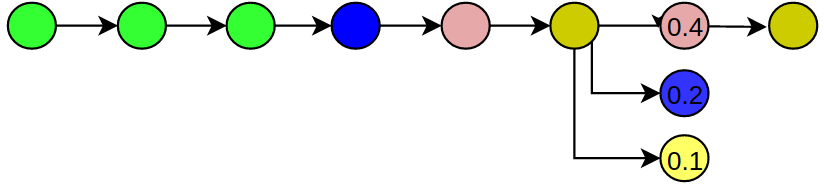
\includegraphics[scale=0.35]{nocycle-algo-1.png}
		\caption{How the next event is chosen}
		\label{figure:nocycle1}	
	\end{center}
\end{figure}

\begin{figure}[!ht]
	\begin{center}  
		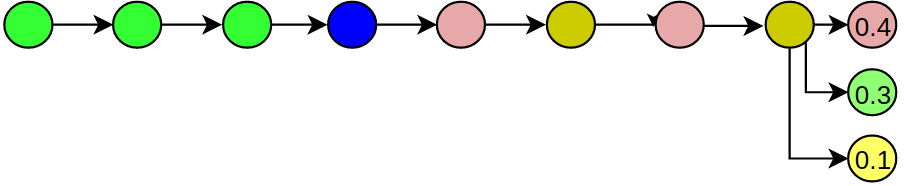
\includegraphics[scale=0.35]{nocycle-algo-2.png}
		\caption{How the next even standardly chosen (cycles present)}
		\label{figure:nocycle2}	
	\end{center}
\end{figure}

\begin{figure}[!ht]
	\begin{center}  
		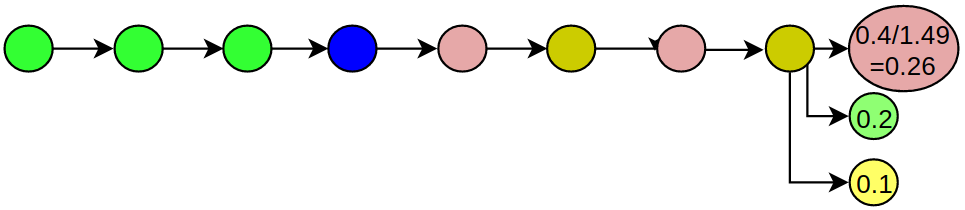
\includegraphics[scale=0.35]{nocycle-algo-3.png}
		\caption{Next event chosen after the $e^{2}$ applied for cycle size 2}
		\label{figure:nocycle3}	
	\end{center}
\end{figure}

\begin{figure}[!ht]
	\begin{center}  
		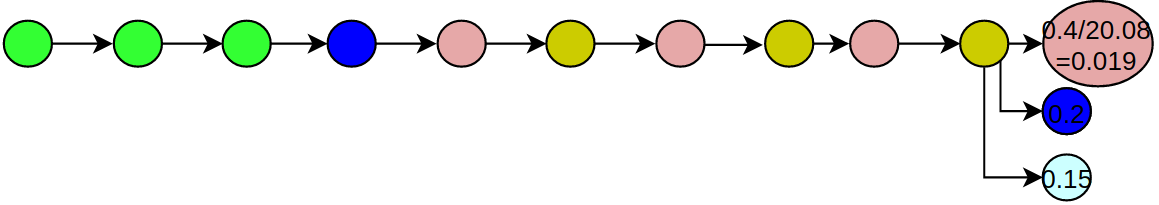
\includegraphics[scale=0.35]{nocycle-algo-4.png}
		\caption{Next event chosen after the $e^{2}$ applied for cycle size 3}
		\label{figure:nocycle4}	
	\end{center}
\end{figure}

Algorithm~\ref{alg:nocycle} reports the pseudo-code of the \nocycle technique. Similarly to Algorithm~\ref{alg:baseline} presented in Section~\ref{subsec:RNNforpredictive}, it takes as input a prefix $p_k(\sigma)$,  the trained LSTM model $lstm$, and the maximum number $max$ of iterations allowed. Then, it returns as output the complete trace (the prefix and the predicted suffix).  In particular, the algorithm adds to the state-of-the-art Algorithm~\ref{alg:baseline} the \textsc{weakenProb} procedure described above to find cycles in the trace and decrease the probability of the first activity of the cycle to occur again at the end of a repetition. The resulting vector of weakened probabilities is hence used for getting the next symbol as in the basic procedure.
%\todocdf{Remember to mention which formula we are using for the evaluation in the evaluation.}

\begin{algorithm}
%\scriptsize
	\caption{\nocycle extension for predicting the suffix of $p_k(\sigma)$}
	\begin{algorithmic}[1]
		\Function{PredictSuffixNoCycle}{$p_k(\sigma)$, $lstm$, $max$}
		\State $k$ = 0
		\State $trace$ = $p_k(\sigma)$
		\Do
		\State $trace_{encoded}$ = \textsc{encode}($trace$)
		\State $next\_symbol\_prob$ = \textsc{predictNextSymbols}($lstm$, $trace_{encoded}$)
		%\State $weakeaning\_coefficient$, $a_{c_1}$ = \textsc{computeWeakeningCoefficient}($trace$)
		\State $weak\_next\_symbol\_prob$ = \textsc{weakenProb} ($trace$, $next\_symbol\_prob$)
		\State $next\_symbol$ = \textsc{getSymbol}($weak\_next\_symbol\_prob$, $trace_{encoded}$)
		%\State $next\_symbol$ = getSymbolAmplified( $next\_symbol\_probabilities$ ,$amplifier$,$symbStartSycle$)
		\State $trace$ = $trace$ $\cdot$ $next\_symbol$
		\State $k$ = $k + 1$
		\doWhile{$($not $next\_symbol$ $==$ $end\_symbol)$ and $(k < max)$}
		\State \textbf{return} trace
		\EndFunction
		
%		\Function{amplify}{$trace$}
%	  \State $rep$ = findAllCycles($trace$)
%		\State \If{$rep$ contains curreny cycle in $trace$} {
%		\State numberOfRep = getNumberCurrentcycleRepeats($rep$,$trace$)
%		\State return amplifyFormula(numberOfRep), firstSymbolOfCurrentTrace}
%		\State return
%		\EndFunction

	%	\Function{getSymbolAmpl}{$nextSymbolProb$, $amplifier$,$symbStartSycle$}
	%	\State index = findItemIndex($symbStartSycle$)
	%	\State $nextSymbolProb$.item(index) = $nextSymbolProb$.item(index) * $amplifier$
	%	\State top = chooseMaxProb($nextSymbolProb$)
	%	\State return probabilityToSymbol(top)
	%	\EndFunction
	\end{algorithmic}
	\label{alg:nocycle}
\end{algorithm}


\subsection{Learning from A-priori Knowledge}
\label{ssec:apriori}

The overall idea for leveraging a-priori knowledge for predictive monitoring is simple: (i) we use the LSTM approach to get the possible predictions for an ongoing trace; this can be done, because the step by step output of a recurrent neural network is basically a probability distribution over next events in the trace. (ii) we rank them according to the likelihood of the prediction; and (iii) we select the first prediction which is compliant with the LTL rules describing the a-priori knowledge. However, although RNN inference algorithms are not computationally expensive per se, building all the possible predicted suffixes could be costly and inefficient. It is the standard problem of algorithms that rely on storing data in tree structures, where the growth of a tree is exponential. That is exactly the case here, independently of how many continuations of the trace are chosen at each step (let's day $N$ steps), each next step of predictions will produce $N^{i}$ nodes. Even for few iterations it is computationally and memory-wise not feasible to use this strategy.

Therefore, the alternative investigated in this paper leverages, on top of state-of-the-art LSTM techniques, the approach classically used in statistical sequence-to-sequence predictions in translation tasks~\cite{Tillmann2003WRD778822778827}, i.e., the \textit{beamSearch} algorithm. The beamSearch works by the partial ordering of the probability trees, that is by exploring the search space, only taking the most promising branches. (As explained in section~\ref{beam-search})
In particular, we use the RNN architecture with LSTM cells and training system proposed in~\cite{niek96732}. Then, in the testing phase, to predict a certain suffix, we use a new inference algorithm (\protrack), which explores the probability space using beamSearch to cut the branches of the LSTM model which bring to predictions that are not compliant with the a-priori knowledge.
% (described in terms of LTL rules).

% The \protrack algorithm has been designed by modifying the inference Algorithm~\ref{alg:baseline} (presented in Section~\ref{sec:background}) to enable the breadth first beamSearch.
%For beamSearch we need to save the probability distribution over most probable of size of beam coefficient.
%\todocg{I've removed the sentence saying that protrack is built on top of \cite{niek96732} because it was already said two lines above.}
Algorithm~\ref{alg:protrack} reports the pseudo-code describing the \protrack algorithm. It takes as input the prefix $p_k(\sigma)$, the available a-priori knowledge $\cal{K}(\sigma)$, and the trained LSTM model $lstm$, together with three parameters: (i) $bSize$, which is the number of possible next symbols returned by algorithm (limiting parameter for a beam search inside of A-PRIORI procedure); (ii) $maxSize$, which is the maximum number of branches that can be explored by \protrack at the same time; and (iii) $max$, which is the maximum number of allowed iterations.

\begin{algorithm}
	\caption{\protrack algorithm for predicting the suffix of $p_k(\sigma)$}
	\label{alg:protrack}
	\begin{algorithmic}[1]
		\Function{\protrack}{$p_k(\sigma)$, $\cal{K}(\sigma)$, $lstm$, $bSize$, $maxSize$, $max$}
		\State $h$ = 0
		\State $prefixes$ = \{$p_k(\sigma)$\}\label{lst2:initialization}
		\While {$k \leq max$ and not \textsc{empty}($prefixes$)} \label{lst2:while}
			\State $candidates\_next$ = \textsc{predictPrefNextSymbols}($lstm$, $prefixes$, $bSize$) \label{lst2:prediction}
			\State $top\_candidates$ = \textsc{topRank}$(candidates\_next$, $maxSize)$ \label{lst2:top}
			\ForAll {$candidate$ in $top\_candidates$} \label{lst2:forall}
%				\If {\textsc{check}$(candidate$, $\cal{K})$} \label{lst2:compliant}
				%	\State $trace$ = \textsc{predictSuffix}$(candidate)$ \label{lst2:predictsuffix}
			%		\State \textbf{return} $trace$
%				\Else
					\If {\textsc{last\_symbol}($candidate$) $<>$ $end\_symbol$}
						\State \textsc{push}($candidate$, $prefixes$)
\Else
					\If {\textsc{check}$(candidate$, $\cal{K})$} \label{lst2:compliant}
\State \textbf{return} $candidate$

\EndIf
				\EndIf
			\EndFor
			\State $h = h + 1$
		\EndWhile
		\EndFunction
	\end{algorithmic}
\end{algorithm}


%Intuitively, the algorithm iterates over a priority queue of prefixes, which is initialized with the input prefix $p_k$ (line~\ref{lst2:initialization}) and that is used for regulating the number of branches to be explored. At the first step, by leveraging the the $bSize$ next events are predicted for the prefix $p_k$ and $bSize$ new traces obtained by concatenating $p_k$ and each of the $bSize$ predicted next events

%If, at the first step, any of the prefixes of the queue is compliant to the formula, the next step consists of predicting for each prefix $p_k$ in $prefixes$ the $bSize$ next events and obtaining $bSize$ new traces by concatenating $p_k$ and each of the $bSize$ predicted next events. So, the algorithm will deal with $\|prefixes\|*bSize$ traces. However, in order to limit the search space, the algorithm ranks the predicted traces based on their estimated probability\footnote{Note that, in order to prevent overflow in the computation, the estimated probability for sequences of events is usually computed as the sum of the log probability (the logarithm of the probability) of the next events probability rather than as the product of the next events probability.} and only takes the top $maxSize$ traces.
%The algoirhtm is iterated until the queue is empty or the maximum number of iterations $max$ is reached (line \ref{lst2:prediction}).

%With this approach we limit our search space to a smaller one. This procedure is heuristic, so sometimes, with a beam size it is possible to cut out best, and/or compliant solutions. In real world testing it has been shown that even with beam size set to $3$, almost always the solutions are found.





\begin{figure}[!ht]
	\begin{center}  
		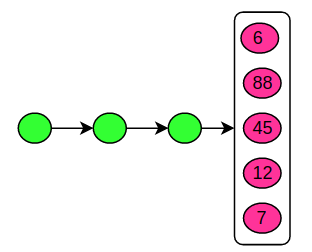
\includegraphics[scale=0.4]{beam-algo-1.png}
		\caption{Beam search based algorithm, step 1}
		\label{figure:beam1}	
	\end{center}
\end{figure}

\begin{figure}[!ht]
	\begin{center}  
		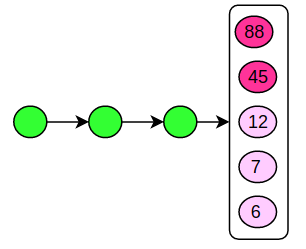
\includegraphics[scale=0.4]{beam-algo-2.png}
		\caption{Beam search based algorithm, step 2}
		\label{figure:beam2}	
	\end{center}
\end{figure}

\begin{figure}[!ht]
	\begin{center}  
		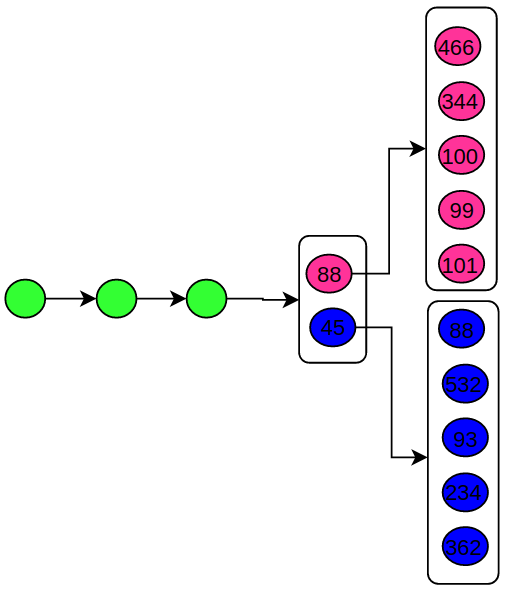
\includegraphics[scale=0.4]{beam-algo-3v2.png}
		\caption{Beam search based algorithm, step 3}
		\label{figure:beam3}	
	\end{center}
\end{figure}

\begin{figure}[!ht]
	\begin{center}  
		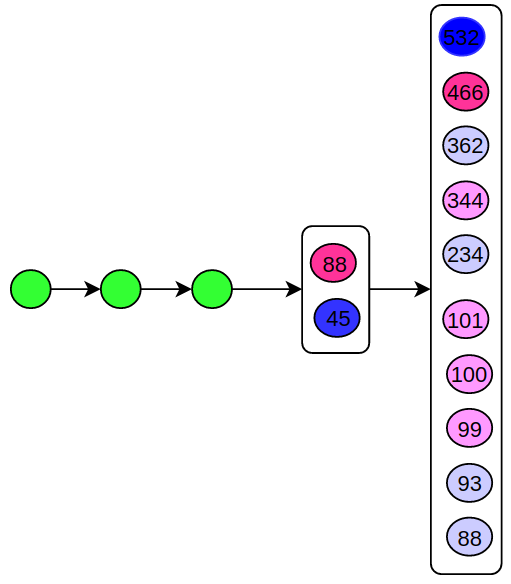
\includegraphics[scale=0.4]{beam-algo-4v2.png}
		\caption{Beam search based algorithm, step 4}
		\label{figure:beam4}	
	\end{center}
\end{figure}

To describe the algorithm we will use the graphics. Figure~\ref{figure:beam1} shows in green the prefix of the trace, and the pink are the 5 predicted next events. Their scores are displayed inside the circles. In the next step (Figure~\ref{figure:beam2}), the algorithm ranks the predicted events and chooses $bSize$ traces (in the exemplary case it's 2). The next step (Figure~\ref{figure:beam3}), predicts the next events for all possible traces saved. Then these traces are combined together in one pool and also ranked with respect to the evaluation function(Figure~\ref{figure:beam4}) and next $bSize$ events are chosen. After the check on the LTL formula approves the predicted sequence, and end symbol is predicted, the process stops, and the sequence is returned (every node keeps a link to its parent node, so reconstruction of the whole trace is not an issue).

Following pseudo code algorithm~\ref{alg:protrack}, the algorithm iterates over a priority queue of prefixes, which is initialized with the input prefix $p_k(\sigma)$ (line~\ref{lst2:initialization}) and that is used for regulating the number of branches to be explored. For each prefix in $prefixes$, $bSize$ ($< maxSize$) possible next activities are predicted (by means of the \textsc{predictNextSymbols} procedure of Algorithm~\ref{alg:baseline}) and for each prefix $bSize$ new traces are obtained by concatenating the prefix with the corresponding $bSize$ predicted next activities (line 5). In this way, the algorithm generates $\left|prefixes\right|*bSize$ traces. In order to limit the search space, the algorithm ranks the predicted traces based on their estimated probability\footnote{Note that, in order to prevent overflow in the computation, the estimated probability for sequences of activities is computed as the sum of the logarithm of the probabilities of the next activities rather than as the product of the probabilities of the next activities.} and takes only the top $maxSize$ ones (line 6). For each of these traces (line 7), if the last symbol predicted is not the end symbol, the trace is added to $prefixes$ (line 9). Otherwise, if the trace is complete, the algorithm checks if it is compliant with the LTL rules in $\cal{K}(\sigma)$ (line 11). In this case, the trace is returned (line 12).
%In the next step, the procedure is iterated.
%the $bSize$ possible next activities are computed and $bSize$ new traces obtained, so that the algorithm will deal with $\left|prefixes\right|*bSize$ traces. At this point, in order to limit the search space, the algorithm ranks the predicted traces based on their estimated probability\footnote{Note that, in order to prevent overflow in the computation, the estimated probability for sequences of activities is computed as the sum of the logarithm of the probabilities of the next activities rather than as the product of the probabilities of the next activities.} and takes only the top $maxSize$ traces.
The algorithm is then iterated until the queue of prefixes is empty or the maximum number of iterations $max$ is reached (line 4).
%This procedure, although ensuring a reduced search space (limited to $maxSize$ nodes to be explored) is a heuristic procedure. Therefore, too low values of $bSize$ can possibly cut out good solutions.
%In real world settings, however, it has been shown that a $bSize$ of $3$ is sufficient to avoid this problem.


%The algorithm builds a priority queue of current prefixes, which at the first iteration only contains the prefix $p_k$ , and uses it as a priority queue for regulating the maximum number of branches to be explored that are active in parallel. It hence loops on such a structure until the queue $prefixes$ is empty or the maximum number of iterations $max$ is reached (line \ref{lst2:prediction}).
%The function \textsc{predictPrefixesNextSymbols} returns, by leveraging the \textsc{predictNextSymbols} procedure of Algorithm~\ref{alg:baseline} and the beam Search algorithm, for each prefix in the queue $prefixes$ of length $\hat{k}_i$, $biSize$ traces of length $\hat{k}_{i+1}$, obtained by concatenating $p_{\hat{k}}$ and the predicted next symbols. All the returned traces of length $\hat{k}_{i+1}$ are then ranked and only the top $maxSize$ are taken \ref{lst2:top}, to guarantee that not too many branches are explored in parallel. For each candidate trace, its compliance with respect to the a-priori knowledge  $\cal(K)$ is checked. If the trace is already compliant to $\cal{K}$, the predictSuffix procedure of Algorithm~\ref{alg:baseline} is invoked and the prediction returned, otherwise, if $p_{\hat{k}_{i+1}}$ has not yet reached the end symbol, the new prefix is added to the $prefixes$ priority queue.


%The algorithm first explores the N next activities given the prefix, and checks if any of them are compliant. If any of them are, the algorithm predicts the remaining trace to the end, assuming to be most probable. If on the first step the LTL formula compliant prefix not found, the next step consists of predicting for every N prefixes N next activities. So it will have $N*N$ resulting traces. The algorithm then decides to cut $N*N-N$ traces based on the estimated probability. It is done by summing up the log probability of the trace up to the last step.

The method \protrack used in the evaluation is the initial algorithm combined with the \nocycle algorithm. To incorporate the \nocycle technique in the algorithm~\ref{alg:protrack}, line 5 method \textit{predictPrefNextSymbol} is updated to account for the cycle removal. Before returning \textit{candidates\_next} the current prefix is analyzed, and if a cycle is found, the next candidates with changed probabilities are returned. 







\subsection{Implementation}
\label{ssec:implementation}
Algorithms~\ref{alg:nocycle} and~\ref{alg:protrack} have been implemented in Python 2.6. In particular, the Keras~\cite{chollet2015keras} and TensorFlow~\cite{tensorflow2015-whitepaper} libraries have been used for neural networks. The LTL checker~\cite{vanderAalst2005} for checking the compliance of traces to LTL rules is instead based on automata and written in Java~\cite{Westergaard2040296}\footnote{The LTL checker is taken from the open source code of ProM process mining suite.}). As the problem of compatibility arose having Java and Python parts, the Py4J library\cite{py4j} was used as a gateway to access Java code from Python. The full source code is available on github\footnote{\url{https://github.com/yesanton/Process-Sequence-Prediction-with-A-priori-knowledge}}. The link given contain detailed readme with instruction on how to reproduce all experiments on any machine. 

%
%When building the \textit{first-best Beam search}, the tree structure was introduced that holds all necessary intermediate values, and up to N leaves. It stores the prefix up to now, parent node (for backtracking), the encoded data, total predicted time, and node status that can be discovered or closed.
%
%The node structure then used to save all path of predictions, and if the execution of the algorithm discovers that at the end the predicted trace is not compliant it starts backtracking to the first non closed node.
%
%For the breath first search the Queue class from Python library was used to store step-wise most probable outcomes.
%
%More implementation details can be seen on our github page.





%%% Local Variables:
%%% mode: latex
%%% TeX-master: "BPM17"
%%% End:

%!TEX root = ./BPM17.tex

\section{Evaluation} % (fold)
\label{sec:evaluation}
%%%% CONTENT

In this section, we provide an evaluation of our predictive business process monitoring techniques based on a-priori knowledge. In particular, we check: (i) whether the \nocycle algorithm leveraging knowledge about the structure of the process execution traces (and in particular about the presence of cycles) actually improves the predictions; and (ii) whether the \protrack algorithm is able to leverage a-priori knowledge to improve the performance of the LSTM model.

\subsection{Event Logs}
\label{ssec:datasets}
%presentation of <datasets, constraints>

\begin{table}[t]
	\centering
	 \begin{scriptsize}
	\begin{tabular}{l|c|c|c|c|c}
		\toprule
			   %  & 		         		     & 		               & %\multicolumn{3}{c}{\textbf{Average}} \\ \cmidrule{5-7}
		\textbf{Log} &\textbf{\#Tr.}  & \textbf{\#Act.}  & \textbf{avg-TL} & \textbf{avg-CR}  & \textbf{Spars.}\\
		\midrule
		EnvLog      & 937    & 299   & 41      & 0.14 & 0.3191 \\
		HelpDesk    & 3804   & 9     & 3.6       & 0.22 & 0.0024 \\
		BPIC11       & 1\,143    & 355   & 54       & 5.05 & 0.3897 \\
		BPIC12       & 13\,087   & 7     & 7.5     & 1.35 & 0.0007 \\
		BPIC13       & 7\,554   & 13    & 7       & 1.45 & 0.0017 \\
		BPIC17       & 31\,509  & 27    & 18     & 0.46 & 0.0009 \\
		\bottomrule
	\end{tabular}
	\end{scriptsize}
	\caption{The event logs}
	\label{table:dataset}
\end{table}

For the evaluation of the techniques, we used six real-life event logs. Four of them were provided for the BPI Challenges (BPIC) 2011~\cite{bpichallenge2011}, 2012~\cite{bpichallenge2012}, 2013~\cite{bpichallenge2013}, and 2017~\cite{bpichallenge2017}, respectively. We also used two additional event logs, one pertaining to an environmental permit application process (``WABO''), used in the context of the CoSeLoG project~\cite{EnvironmentalLog} (\emph{EnvLog} for short in this paper), and another containing cases from a ticketing management process of the help desk of an Italian software company (\emph{Helpdesk}\footnote{\url{https://data.mendeley.com/datasets/39bp3vv62t/1}} for short).

\begin{enumerate}
	\item \textbf{Environment permit log} (\emph{EnvLog}) is the log containing data that come from Dutch municipality\footnote{\url{https://data.4tu.nl/repository/uuid:e8c3a53d-5301-4afb-9bcd-38e74171ca32}}. The cases are the application process of the environment permits. It contains 937 cases, 38.944 events, and 381 events types.
	\item \textbf{Helpdesk} is the dataset containing events from a ticketing management process of the help desk of an Italian software company. The process consists of 9 activities, and all cases start with the insertion of a new ticket into the ticketing
	management system. Each case ends when the issue is resolved and the ticket is closed. This log contains 3804 process instances (a.k.a "cases") and 13710 events
	\item \textbf{BPI 11 log} is the famous in process mining log taken from Dutch Academic Hospital. The cases of the log correspond to the Gynaecology department of the hospital. Phases consist of the diagnosis and treatment of the patient. Some attributes are repeating as the procedures could take place few number of times. As the log contains sensitive information it was anonymized.
	\item \textbf{BPI 12 subprocess W dataset\footnote{\url{http://data.4tu.nl/repository/uuid:3926db30-f712-4394-aebc-75976070e91f}.}} This is the part of the BPI 2012 challenge, that contains a real-life log, taken from a Dutch Financial Institute. The process represented in the event log is an application process for a personal loan or overdraft within a global financing organization. 
	
	This log is contains a lot of information the usual prediction task system would bot be interested in. The paper\cite{niek96732} proposed to cut the log down to the traces what contain events that are manualy executed. So the pre-processed log was taken from their github repository\footnote{\url{https://github.com/verenich/ProcessSequencePrediction/tree/master/data}}.
	
	\item \textbf{BPI 13 log\footnote{\url{http://www.win.tue.nl/bpi/doku.php?id=2013:challenge}}} was prepared by Volvo IT in Belgium. Log consist of incident and problem management from their system "VINST".   
	
	\item \textbf{BPI 17 log\footnote{\url{http://data.4tu.nl/repository/uuid:5f3067df-f10b-45da-b98b-86ae4c7a310b}}} is a process taken from Dutch financial institute. In particular the process we used it a loan applications. It has much more data that other logs that we considered. 
		
	
\end{enumerate}

The characteristics of these logs are summarized in Table~\ref{table:dataset}. For each log, we report the total number of traces, the number of activity labels (i.e., the size of the activity set of the log), the average trace length (avg-TL), the average number of repetitions of all cycles in the log (avg-CR), and the ratio between the number of activity labels and the number of traces, indicating the sparsity of the activity labels over the log.
%Concerning the test set we did use 67\% of the whole dataset for training. Then we selected for testing a relevant subset of the remaining 33\%  satisfying, for each dataset, the additional (a-priori) knowledge, described in terms of LTL formulas. To maximize the size of the testing set we selected LTL formulas satisfied by a conspicuous number of traces among the remaining 33\% ones.

%For the a-priori knowledge, we divided the event logs in training and testing set and we selected LTL formulas satisfied by a conspicuous number of traces in the testing set. For each event log we selected a conjunction of \textit{strong} and of \textit{weak} formulas, which respectively strongly and weakly constrain the trace. For instance a formula LTL of the type $\sometime A$ is weaker than a formula $\always(A \imp \sometime B) \wedge \sometime A$ since the latter imposes the occurrence of both $A$ and $B$ and of a temporal relationships between them. The schematic form of the formulas used in the evaluation is reported in Table~\ref{table:apriori}, where - for the sake of readability - we replace the original activity names with propositional atoms.
% reported in Table~\ref{table:apriori} by means of LTL (linear time temporal logic) formulas.


%experiment setup table




\subsection{Experimental Procedure}
\label{ssec:procedure}
%presentation of baseline + metrics



In order to evaluate the techniques presented in the paper, we adopted the following procedure. For each event log:
\begin{enumerate}
%	\item We divided all our event logs in three parts: a \textbf{training set} composed of the 67\% of the whole event log and two \textbf{testing sets}, a so-called strong-apriori testing set and a so-called weak-apriori testing set, respectively composed of the subsets of the remaining 33\% which satisfy the strong and weak a-priori knowledge reported in Table~\ref{table:apriori}\footnote{Note that strong-apriori and weak-apriori are not necessarily disjoint.}.
\item We divided the event log in two parts: a \textbf{training set} composed of the 67\% of the whole event log and a \textbf{testing set}, composed of the remaining 33\%.
\item We derived the a-priori knowledge on the traces of the testing set as follows. We randomly selected 10\% of traces of the testing set. From each trace, we extracted 4 prefixes of lengths corresponding to the 4 integers in the interval $\left[mid-2,mid+2\right]$, where $mid$ is half of the median of the trace lengths. We derived all suffixes of these prefixes and we used the DeclareMiner ProM plug-in~\cite{Maggi2012} to discover LTL rules satisfied in all those suffixes (Figure~\ref{figure:ltl} shows the LTL extraction from DeclareMiner). Then, we defined 2 conjunctive rules describing a \textit{strong a-priori knowledge} and a \textit{weak a-priori knowledge}, which respectively strongly and weakly constrain the traces. In particular, we discovered rules of type $\sometime A$ (which imposes the occurrence of $A$) for defining the weak a-priori knowledge and rules of type $\always(A \imp \sometime B) \wedge \sometime A$ (which imposes the occurrence of both $A$ and $B$ and that every occurrence of $A$ is followed by an occurrence of $B$) for defining the strong a-priori knowledge. For the weak a-priori knowledge, we randomly selected from the discovered rules one, two or three (depending on the average length of the traces in the log) rules of type $\sometime A$ and we composed them into a single conjunctive formula. Similarly, for the strong a-priori knowledge, we randomly selected one, two or three rules from the discovered rules of type $\always(A \imp \sometime B) \wedge \sometime A$ and we composed them into a single conjunctive formula. We followed this systematic procedure for defining the a-priori knowledge, to limit the bias of the selected rules while guaranteeing that they are satisfied in a reasonable number of traces of the testing set. The schematic form of the rules used in the evaluation is reported in Table~\ref{table:apriori}, where - for the sake of readability - we replace the original activity names with single characters. Starting from strong and weak a-priori knowledge, we built a \emph{strong a-priori testing set} and a \emph{weak a-priori testing set}, respectively composed of the subsets of traces of the testing set that satisfy strong and weak a-priori knowledge.

\begin{figure}[!ht]
	\begin{center}  
		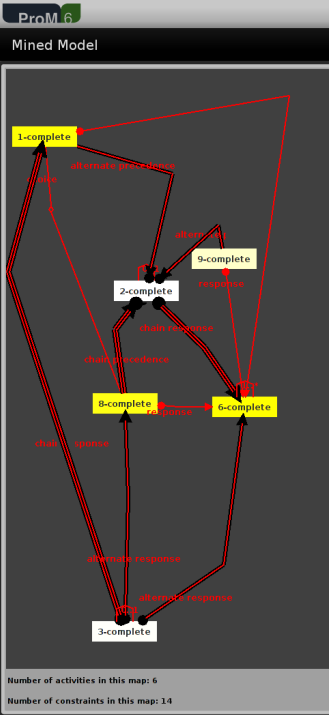
\includegraphics[height=15cm]{3_ltl_prom.png}
		\caption{Declare Miner in action}
		\label{figure:ltl}
	\end{center}
\end{figure}


\item  we compared \nocycle and \protrack \footnote{We set $bSize$ to $3$ and, for the coefficient in charge of weakening the probabilities of activities in a cycle, we used the exponential formula ($e^{j}$, where $j$ is the number of cycle repetitions).} against a baseline provided by the technique presented in \cite{niek96732}. For each technique, we computed: (i) the length of the predicted suffixes; and (ii) their similarity with the prediction ground truth measured using the Damerau-Levenshtein similarity~\cite{Damerau:1964:TCD:363958.363994}.
\end{enumerate}
\begin{table}[t!]
	\centering	
	\begin{scriptsize}
	\begin{tabular}{l|c|c}
		\toprule
		\textbf{Log}  & \textbf{A-priori Strong} & \textbf{A-priori Weak} \\
		\midrule
		EnvLog     & $\always(a \imp \sometime b) \wedge \sometime a \wedge \always(c \imp \sometime d) \wedge \sometime c$  & $\sometime a \wedge \sometime c$ \\
		HelpDesk   & $\always(e \imp \sometime f) \wedge \sometime e$ & $\sometime e$\\
		BPIC11      & $\always(g \imp \sometime h) \wedge \sometime g \wedge \always(i \imp \sometime l) \wedge \sometime i \wedge \always(m \imp \sometime n) \wedge \sometime m$ &
		$\sometime i \wedge \sometime h \wedge \sometime o$		\\
		BPIC12      & $\always(p \imp \sometime q) \wedge \sometime p$ & $\sometime p$   \\
		BPIC13      & $\always(r \imp \sometime s) \wedge \sometime r \wedge \always(t \imp \sometime r) \wedge \sometime t$ & $\sometime s \wedge \sometime r$ \\
		BPIC17      & $\always(u \imp \sometime v) \wedge \sometime u$  & $\sometime u$  \\
		\bottomrule
	\end{tabular}
	\end{scriptsize}
	\caption{The a-priori knowledge.}
	\label{table:apriori}
\end{table}
The experiments have been performed both on a GPU Tesla K40c and on a conventional laptop with Code i5 CPU. As for the LSTM training settings we used the ones identified by Tax et al.~\cite{niek96732} as the most performing ones for facing the problem of predicting sequences of future activities.\footnote{We used an architecture characterized by two LSTM layers. The algorithm used is the Adam learning algorithm with categorical cross entropy loss and the dropout coefficient has been set to 0.2.} The time required for training the LSTM neural network is about 2 minutes per epoch using the GPU and 15 minutes using the CPU. The inference time for \nocycle %(not modified version of LSTM model prediction)
 is about 0.1-2 seconds per trace (depending on the log), whereas the inference time for \protrack is 4 times higher on average.


%We used two hidden layers for the network: one shared layer for sequence of activities and time feature, and two joint layers for activities and time sequence preceding output layer. The dropout coefficient is 0.2, and the network is equipped Adam learning algorithm. These parameters shown to work best for the problem at hand\cite{niek96732}. We also have 500 maximum number of epoch, and categorical cross entropy loss.

\subsection{Results and Discussion}
\label{ssec:results}
%big table of results + comment the table (comment on logs with cycles, comment that and on why protrack traces are longer than backtrack, ... )

Tables~\ref{table:results-strong} and~\ref{table:results-weak} report, for each event log, the performances of the two techniques we propose on the strong a-priori and weak a-priori testing sets. Also, one can take a look at the figure~\ref{figure:results} where results are visualized. The results for both testing sets are compared with the baseline presented in~\cite{niek96732}. For each log, we provide the average Damerau-Levenshtein similarity between the predicted sequence (in square brackets, its average length) and the ground truth (column 5). The best average Damerau-Levenshtein similarity for each log is emphasized in gray. Column 6 reports the number of traces tested while column 7 specifies the range of the prefix lengths used for the specific event log. %The prefixes range is chosen around middle point of the average lengths of the traces.

\newcommand{\maxf}[1]{{\cellcolor[gray]{0.8}} #1}

%\begin{table}[h]
%	\centering
%	\sisetup{detect-weight=true,detect-inline-weight=math}
%	\begin{tabular}{lS[table-unit-alignment = right]s[table-unit-alignment = left]S[table-unit-alignment = right]s[table-unit-alignment = left]S[table-unit-alignment = right]s[table-unit-alignment = left]S[table-unit-alignment = right]s[table-unit-alignment = left]Sc}
%		\toprule
%		\textbf{Log}  & \multicolumn{2}{c}{\textbf{Baseline}} & \multicolumn{2}{c}{\nocycle} & \multicolumn{2}{c}{\backtrack}  & \multicolumn{2}{c}{\protrack} & \textbf{Groundtruth}  & \textbf{Prefix} \\\hline
%		EnvLog        & \maxf{0.22}&[\num{25.99}]   & 0.22&[\num{25.49}]        & 0.22&[\num{26.26}]                            & 0.22&[\num{27.67}]          & 33.61                 & 2-20         \\
%		HelpDesk      & 0.65&[\num{1.26}]           & 0.65&[\num{1.26}]         & \maxf{0.77}&[\num{1.15}]                      & \maxf{0.77}&[\num{1.15}]    & 1.71                  & 2-Max         \\
%		BPI11         & 0.19&[\num{199.00}]         & 0.24&[\num{42.59}]        & \maxf{0.34}&[\num{57.61}]                     & 0.25&[\num{145.86}]         & 89.41                 & 10 \\
%		BPI13         & 0.58&[\num{32.30}]          & \maxf{0.60}&[\num{2.60}]  & 0.57&[\num{1.76}]                             & 0.53&[\num{2.29}]           & 1.92                  & 3-10          \\
%		BPI12         & 0.08&[\num{58.74}]          & 0.26&[\num{2.10}]         & 0.16&[\num{1.33}]                             & \maxf{0.32}&[\num{2.75}]    & 7.22                  & 3-10           \\
%		BPI17         & 0.40&[\num{13.62}]          & 0.40&[\num{13.62}]        & \maxf{0.41}&[\num{13.46}]                     & 0.40&[\num{13.62}]          & 9.39                  & 5        \\
%		\bottomrule
%	\end{tabular}
%	\caption{Results related to predictions.}
%		\label{table:results}
%\end{table}

\begin{table}[t]
	\centering
	\sisetup{detect-weight=true,detect-inline-weight=math}
\begin{scriptsize}
	\begin{tabular}{lS[table-unit-alignment = right]s[table-unit-alignment = left]S[table-unit-alignment = right]s[table-unit-alignment = left]S[table-unit-alignment = right]s[table-unit-alignment = left]S[table-unit-alignment = right]s[table-unit-alignment = right]s[table-unit-alignment = left]Sc}
		\toprule
		\textbf{Log}  & \multicolumn{2}{c}{\textbf{Baseline}} & \multicolumn{2}{c}{\nocycle}  & \multicolumn{2}{c}{\protrack} & \textbf{Groundtruth} & \textbf{Tested} & \textbf{Prefix} \\\hline
		EnvLog        & \maxf{0.250}&[\num{17.4}]   & \maxf{0.250}&[\num{17.4}]                      & 0.070&[\num{95.00}]          & 29.40              & 80   & 19-22         \\
		HelpDesk      & 0.551&[\num{1.44}]           & 0.551&[\num{1.44}]                       & \maxf{0.831}&[\num{2.36}]    & 3.00         & 576         & 2-5          \\
		BPIC11         & 0.204&[\num{199.00}]         & \maxf{0.281}&[\num{199.00}]                      & 0.274&[\num{198.00}]         & 117.11          & 144       & 13-16 \\
		BPIC12         & 0.071&[\num{47.07}]          & 0.387&[\num{6.86}]                       & \maxf{0.416}&[\num{7.53}]    & 10.95          & 1\,548        & 2-5            \\
		BPIC13         & 0.116&[\num{100.80}]          & 0.502&[\num{14.71}]                & \maxf{0.596}&[\num{6.13}]           & 7.15       & 3\,209           & 2-5          \\
		BPIC17         & 0.448&[\num{11.78}]          & 0.448&[\num{11.78}]                      & \maxf{0.510}&[\num{15.14}]          & 16.01        & 10\,153          & 6-9        \\
		\bottomrule
	\end{tabular}
\end{scriptsize}
	\caption{Prediction results on the strong a-priori testing set}
	\label{table:results-strong}
\end{table}


\begin{table}[t]
	\centering
	\sisetup{detect-weight=true,detect-inline-weight=math}
\begin{scriptsize}
	\begin{tabular}{lS[table-unit-alignment = right]s[table-unit-alignment = left]S[table-unit-alignment = right]s[table-unit-alignment = left]S[table-unit-alignment = right]s[table-unit-alignment = left]S[table-unit-alignment = right]s[table-unit-alignment = right]s[table-unit-alignment = left]Sc}
		\toprule
		\textbf{Log}  & \multicolumn{2}{c}{\textbf{Baseline}} & \multicolumn{2}{c}{\nocycle}  & \multicolumn{2}{c}{\protrack} & \textbf{Groundtruth}  & \textbf{Tested} & \textbf{Prefix} \\\hline
		EnvLog        & \maxf{0.246}&[\num{18.22}]   & \maxf{0.246}&[\num{18.22}]                      & 0.084&[\num{89.91}]          & 31.31              & 108  & 19-22         \\
		HelpDesk      & 0.551&[\num{1.44}]           & 0.551&[\num{1.44}]                       & \maxf{0.747}&[\num{2.14}]    & 3.00             & 576    & 2-5         \\
		BPIC11         & 0.220&[\num{199.00}]         & \maxf{0.292}&[\num{199.00}]                      & 0.282&[\num{197.4}]         & 112.66            & 450     & 13-16 \\
		BPIC12         & 0.100&[\num{48.08}]          & 0.263&[\num{6.81}]                       & \maxf{0.264}&[\num{7.00}]    & 8.33       &      3\,179     & 2-5           \\
		BPIC13         & 0.130&[\num{95.19}]          & 0.459&[\num{14.92}]                & \maxf{0.569}&[\num{5.14}]           & 5.85         &  4\,364         & 2-5          \\
		BPIC17         & 0.448&[\num{11.78}]          & 0.448&[\num{11.78}]                      & \maxf{0.469}&[\num{14.00}]          & 16.01        & 10\,153          & 6-9        \\
		\bottomrule
	\end{tabular}
\end{scriptsize}
	\caption{Prediction results on the weak a-priori testing set}
	\label{table:results-weak}
\end{table}



\begin{figure}[!ht]
	\begin{center}  
		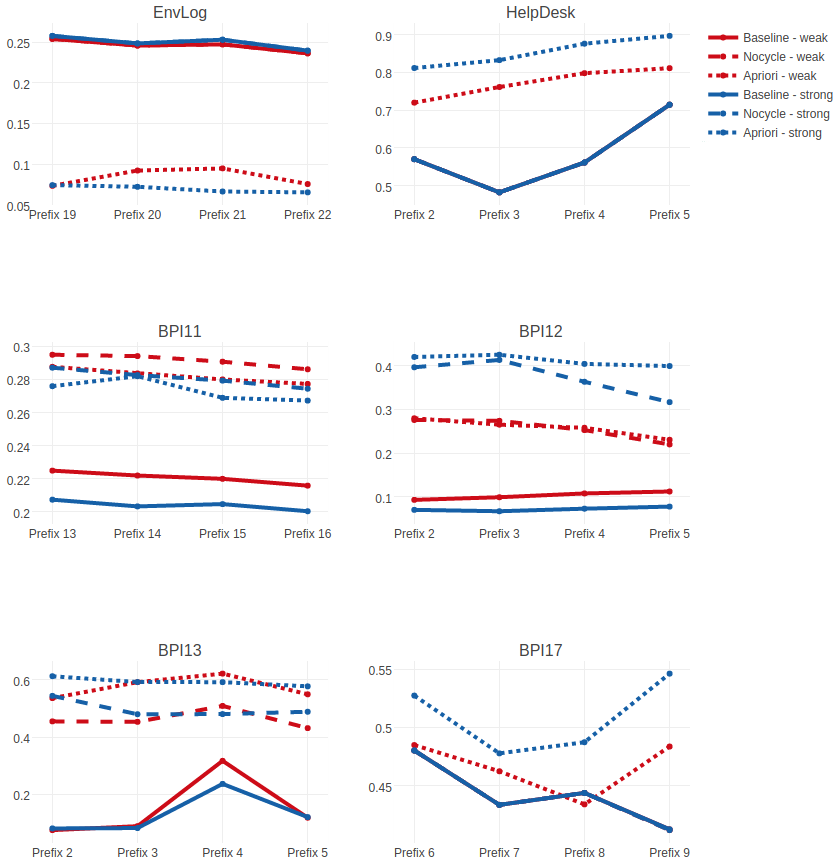
\includegraphics[width=\textwidth]{2_evaluation.png}
		\caption{Graphical representation of evaluation}
		\label{figure:results}
	\end{center}
\end{figure}


The tables show that the proposed algorithms outperform the baseline in most of the logs.
The presence of cycles in the logs has a strong impact on the performance of the \nocycle algorithm. In particular, if the logs have an average number of cycle repetitions smaller than $0.5$, as in the case of EnvLog, HelpDesk and BPIC17, then \nocycle does not show any improvement over the baseline. Therefore, we can conclude that \nocycle correctly deals with the presence of cycles in the logs to improve the predictions.




%Concerning the ability of \protrack to leverage the regularity of the logs, it is evident that the best improvements obtained by the \protrack algorithm refer to event logs that have a small activity set (small number of activity labels) and not HelpDesk and BPIC13 in our experiments.

\protrack perform worse on logs EnvLog and the BPIC11. The reason for this can be explained by the fact that, in these two logs, activity labels are sparse with an unusually high number of labels with respect to the number of traces. Indeed, Table~\ref{table:dataset} shows that the ratio between the number of activity labels and the number of traces (column 8) for these logs is higher with respect to the other logs.
%While a full investigation of the impact of the log characteristics over the performance of LSTM-based techniques is out of the scope for this paper and is left to future work, we can already say that logs characterized by a high degree of sparsity of activity labels (and, therefore, containing sparse behaviors) are unlikely candidates to benefit from the proposed techniques.
We can also notice that the availability of highly constraining rules in the a-priori knowledge improves the performance of \protrack. Therefore, we can conclude that \protrack is able to correctly leverage a-priori knowledge in a way that it performs better when the activity set of the log is not particularly large (and the log does not contain sparse behaviors) and when the a-priori knowledge constrains more the process behavior.




%To sum up, the evaluation shows that both the \nocycle and the \protrack techniques actually improve the performance of the baseline approach and they are particularly suitable to be used when the event logs present several cycles or when the alphabet is not extremely large, respectively.

% , we can observe
% 	\item {Big performance for apriori shown on logs which have small alphabet and not much cycles (helpdesk, bpi13)}
% 	\item {For logs mentioned above and for the same reasons, the difference between STRONG and WEAK formulas are bigger(STRONG performs very good). }
% 	\item {Applying STRONG formulas gives better results as they more constraining in most cases.}


%\todoincg{shall we add a sentence in terms of lessons learned or is this enough?}
% \subsection{Discussion}
%
% \begin{itemize}
% 	% \item{Environment permit, BPI11 do not improve with apriori knowledge because the training data is too sparse and alphabet size is too big.}
% 	% \item{If there are no cycles (in our logs it is less than 0.5 per trace) there is no improvement for NOCycle technique. (Examples env permit, helpdesk, bpi17)}
% 	\item {Big performance for apriori shown on logs which have small alphabet and not much cycles (helpdesk, bpi13)}
% 	\item {For logs mentioned above and for the same reasons, the difference between STRONG and WEAK formulas are bigger(STRONG performs very good). }
% 	\item {Applying STRONG formulas gives better results as they more constraining in most cases.}
%
% \end{itemize}

% \label{ssec:discussion}
% "lessons learned"': when we have cycles in the log, we should use the cycle approach, when the average lenght of the log is high then use protrack, ...

% section evaluation (end) 
%!TEX root = ./BPM17.tex

\section{Conclusions} % (fold)
\label{sec:conclusions}

%In this paper we have presented a family of techniques presented in this paper, together with their careful evaluation, aims at addressing the insertion of apriori knowledge in predictive business process monitoring algorithms. Our contribution is twofold. In Section~\ref{sec:our_approach} have three techniques based on Recurrent Neural Networks (RNN) able to leverage knowledge on the dataset structure as well as apriori knowledge for predicting the sequence of future activities in ongoing traces, while in Section~\ref{sec:evaluation} we have shown that taking into account the dataset structure as well as the apriori knowledge increases the accuracy of the results over a plain RNN-based baseline.
In the thesis, we have presented two techniques based on RNNs with LSTM cells able to leverage knowledge about the structure of the process execution traces as well as a-priori knowledge about their future development for predicting the sequence of future activities of an ongoing case. In particular, we show that opportunely tailoring LSTM-based algorithms it is possible to take into account a-priori knowledge at prediction time without the need to retrain the predictive algorithms in case new knowledge becomes available. The results of our experiments show that \nocycle correctly deals with the presence of cycles in the logs and \protrack is able to correctly leverage a-priori knowledge in a way that it performs better with logs characterized by a low degree of sparsity of activity labels and when the a-priori knowledge constrains the behavior of the process more.

Future work will include: (i) dealing with more complex forms of a-priori knowledge. In particular, we aim at addressing a-priori knowledge on activities and on their data payload, as well as the dynamic knowledge that can evolve in the future of an ongoing case; that might include other ways of representing the knowledge. It might be possible to extend LTL rules with some case specific semantics;  (ii) extending the proposed algorithms to leverage a-priori knowledge also for other types of predictions; (iii) extending the experimental evaluation especially focusing on the investigation of metrics for evaluating the influence on the predictions of the different degrees of freedom/strength of the a-priori knowledge; and (iv) inserting the presented techniques in predictive business process monitoring frameworks such as the one discussed in~\cite{Di-Francescomarino:2016aa}. 

\newpage

% section conclusions (end) 


\bibliographystyle{splncs03}
\bibliography{bibliography}

\end{document}

%%% Local Variables:
%%% mode: latex
%%% TeX-master: t
%%% End:
